\documentclass[sigconf]{acmart}
\AtBeginDocument{%
  \providecommand\BibTeX{{%
    Bib\TeX}}}

%% Rights management information.  This information is sent to you
%% when you complete the rights form.  These commands have SAMPLE
%% values in them; it is your responsibility as an author to replace
%% the commands and values with those provided to you when you
%% complete the rights form.
\setcopyright{acmcopyright}
\copyrightyear{tbd}
\acmYear{tbd}
\acmDOI{tbd}

%% These commands are for a PROCEEDINGS abstract or paper.
\acmConference[Conference acronym 'XX]{Make sure to enter the correct conference title from your rights confirmation emai}{tbd}{tbd}
%%
%%  Uncomment \acmBooktitle if the title of the proceedings is different
%%  from ``Proceedings of ...''!
%%
%%\acmBooktitle{Woodstock '18: ACM Symposium on Neural Gaze Detection,
%%  June 03--05, 2018, Woodstock, NY}
\acmISBN{978-1-4503-XXXX-X/18/06}


%%
%% Submission ID.
%% Use this when submitting an article to a sponsored event. You'll
%% receive a unique submission ID from the organizers
%% of the event, and this ID should be used as the parameter to this command.
%%\acmSubmissionID{123-A56-BU3}

%%
%% For managing citations, it is recommended to use bibliography
%% files in BibTeX format.
%%
%% You can then either use BibTeX with the ACM-Reference-Format style,
%% or BibLaTeX with the acmnumeric or acmauthoryear sytles, that include
%% support for advanced citation of software artefact from the
%% biblatex-software package, also separately available on CTAN.
%%
%% Look at the sample-*-biblatex.tex files for templates showcasing
%% the biblatex styles.
%%

%%
%% The majority of ACM publications use numbered citations and
%% references.  The command \citestyle{authoryear} switches to the
%% "author year" style.
%%
%% If you are preparing content for an event
%% sponsored by ACM SIGGRAPH, you must use the "author year" style of
%% citations and references.
%% Uncommenting
%% the next command will enable that style.
%%\citestyle{acmauthoryear}


%%
%% end of the preamble, start of the body of the document source.


\usepackage{amsmath,amsfonts}
\usepackage{amsthm}
\usepackage{algorithm,algpseudocode,float}
\usepackage{lipsum}
\usepackage{multicol}
\usepackage{cleveref}
\usepackage{fancybox}
\usepackage{makecell}
\usepackage{arydshln}
%\usepackage{subfigure}
\usepackage{subfig}
%\usepackage{subcaption}
\usepackage{multirow}
\usepackage{threeparttable}
\usepackage{autobreak}
\allowdisplaybreaks
    
%% New commands goes here
\newcommand{\Enote}[1]{\color{purple}Enote: #1\color{black}}
\newcommand{\Yaxin}[1]{\color{brown}Yaxin: #1\color{black}}
\newcommand{\Niv}[1]{\color{blue}Niv: #1\color{black}}

\newcommand{\Gen}{{\sf Gen}}
\newcommand{\Eval}{{\sf Eval}}
\newcommand{\FullEval}{{\sf FullEval}}
\newcommand{\Conv}{{\sf Conv}}
\newcommand{\conv}{{\sf conv}}
\newcommand{\CW}{{\sf CW}}
\newcommand{\Correct}{{\sf Correct}}
\newcommand{\Encode}{{\sf Encode}}
\newcommand{\Decode}{{\sf Decode}}
\newcommand{\Position}{{\sf Position}}
\newcommand{\Schedule}{{\sf Schedule}}
\newcommand{\Expand}{{\sf Expand}}
\newcommand{\row}{{\sf row}}
\newcommand{\seed}{{\sf seed}}
\newcommand{\sign}{{\sf sign}}
\newcommand{\res}{{\sf res}}
\newcommand{\correct}{{\sf correct}}
\newcommand{\map}{{\sf map}}
\newcommand{\stat}{{\sf stat}}
\newcommand{\poly}{{\sf poly}}
\newcommand{\Adv}{{\sf Adv}}
\newcommand{\MULT}{{\sf MULT}}
\newcommand{\Hyb}{{\sf Hyb}}

\newcommand{\DMPF}{{\sf DMPF}}
\newcommand{\DPF}{{\sf DPF}}
\newcommand{\OKVS}{{\sf OKVS}}
\newcommand{\LPN}{{\sf LPN}}
\newcommand{\CBC}{{\sf CBC}}
\newcommand{\PBC}{{\sf PBC}}
\newcommand{\PCG}{{\sf PCG}}
%rule: specific parametrized objects in \sf, other in text terminologies in \rm. 
    
\newcommand{\GG}{\mathbb{G}}
\newcommand{\NN}{\mathbb{N}}
\newcommand{\ZZ}{\mathbb{Z}}
\newcommand{\FF}{\mathbb{F}}

\newcommand{\cA}{\mathcal{A}}
\newcommand{\cHW}{\mathcal{HW}}
\newcommand{\cRHW}{\mathcal{RHW}}
\newcommand{\cC}{\mathcal{C}}

\newcommand{\red}[1]{\textcolor{red}{#1}}
\newcommand{\ipd}[2]{\langle #1, #2 \rangle}

\newtheorem{theorem}{Theorem}
\newtheorem{lemma}[theorem]{Lemma}
\newtheorem{claim}[theorem]{Claim}
\newtheorem{fact}[theorem]{Fact}
\newtheorem{definition}[theorem]{Definition}
\newtheorem{example}[theorem]{Example}
\newtheorem{remark}[theorem]{Remark}
\newtheorem{construction}{Construction}
\newtheorem{corollary}[theorem]{Corollary}
\newtheorem{proposition}[theorem]{Proposition}

\makeatletter
\newcommand{\algorithmfootnote}[2][\footnotesize]{%
  \let\old@algocf@finish\@algocf@finish% Store algorithm finish macro
  \def\@algocf@finish{\old@algocf@finish% Update finish macro to insert "footnote"
    \leavevmode\rlap{\begin{minipage}{\linewidth}
    #1#2
    \end{minipage}}%
  }%
}
\makeatother
%%

\begin{document}

%%
%% The "title" command has an optional parameter,
%% allowing the author to define a "short title" to be used in page headers.
\title{Notes for New Constructions of DMPF}

\author{tbd}
\authornote{Both authors contributed equally to this research.}
\email{tbd}
\orcid{tbd}
\author{tbd}
\authornotemark[1]
\email{tbd}
\affiliation{%
  \institution{tbd}
  \streetaddress{tbd}
  \city{tbd}
  \state{tbd}
  \country{tbd}
  \postcode{tbd}
}

\author{tbd}
\affiliation{%
  \institution{tbd}
  \streetaddress{tbd}
  \city{tbd}
  \country{tbd}}
\email{tbd}

%%
%% By default, the full list of authors will be used in the page
%% headers. Often, this list is too long, and will overlap
%% other information printed in the page headers. This command allows
%% the author to define a more concise list
%% of authors' names for this purpose.
\renewcommand{\shortauthors}{tbd et al.}

\begin{abstract}
  tbd. 
\end{abstract}

%%
%% The code below is generated by the tool at http://dl.acm.org/ccs.cfm.
\begin{CCSXML}
  <ccs2012>
     <concept>
         <concept_id>10003752.10003777.10003788</concept_id>
         <concept_desc>Theory of computation~Cryptographic primitives</concept_desc>
         <concept_significance>500</concept_significance>
         </concept>
   </ccs2012>
\end{CCSXML}
  
\ccsdesc[500]{Theory of computation~Cryptographic primitives}

%%
%% Keywords. The author(s) should pick words that accurately describe
%% the work being presented. Separate the keywords with commas.
\keywords{tbd}
%% A "teaser" image appears between the author and affiliation
%% information and the body of the document, and typically spans the
%% page.
%\begin{teaserfigure}
  %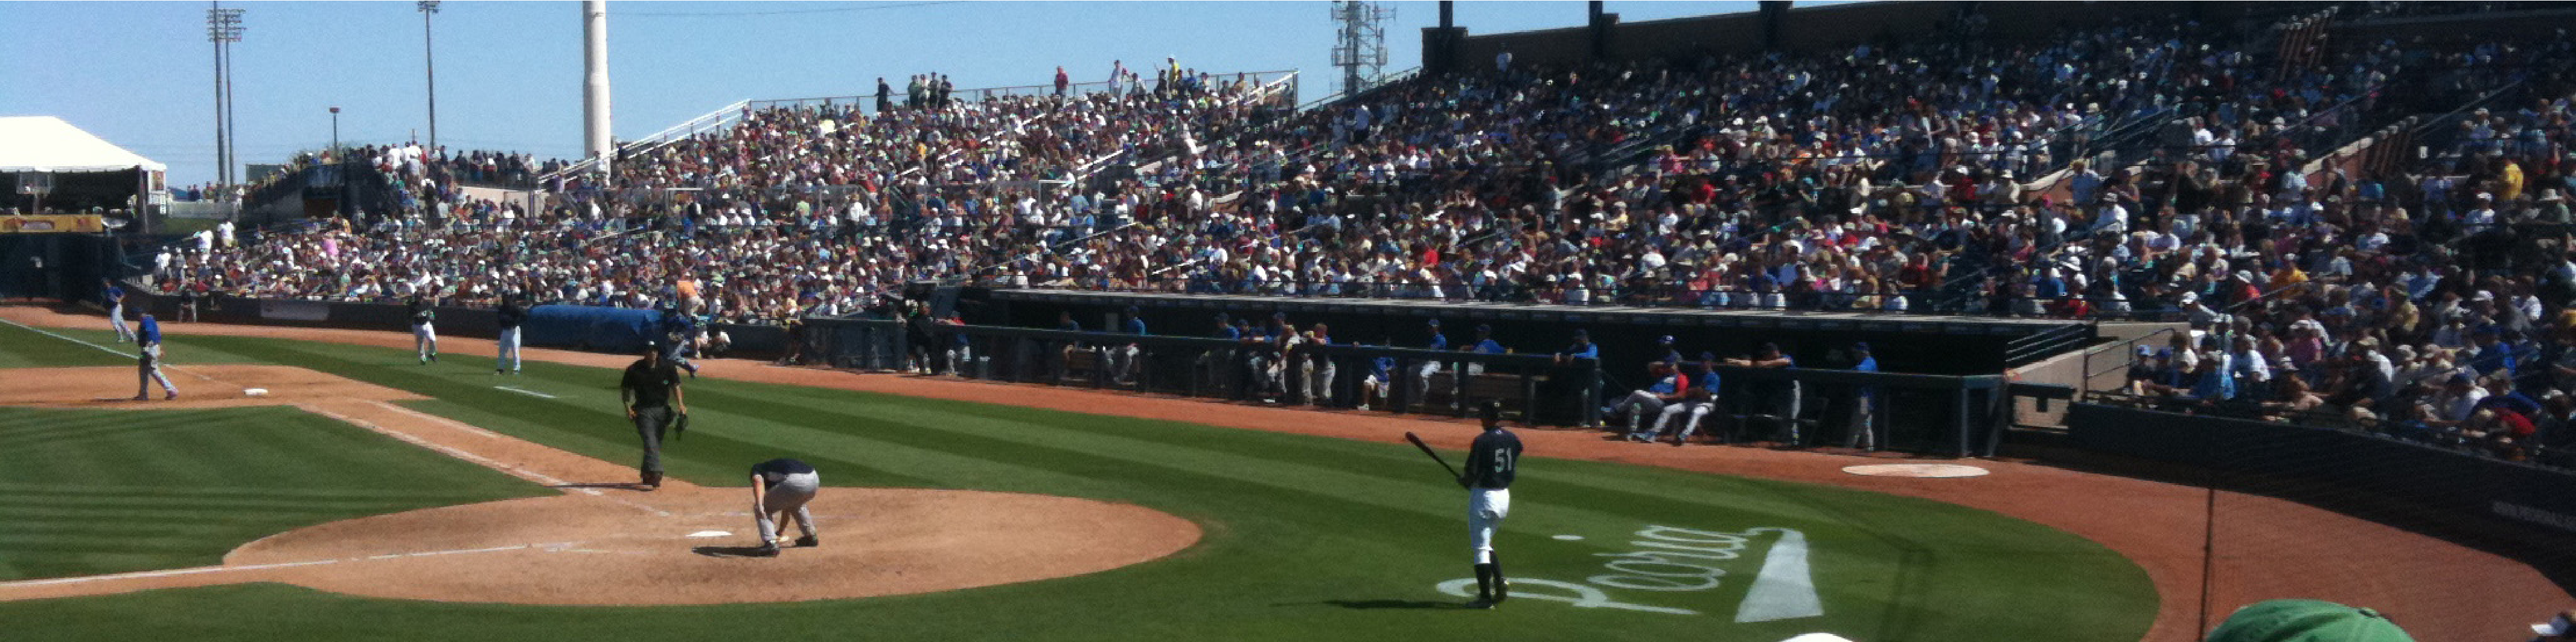
\includegraphics[width=\textwidth]{sampleteaser}
  %\caption{Seattle Mariners at Spring Training, 2010.}
  %\Description{Enjoying the baseball game from the third-base
  %seats. Ichiro Suzuki preparing to bat.}
  %\label{fig:teaser}
%\end{teaserfigure}

\received{20 February 2007}
\received[revised]{12 March 2009}
\received[accepted]{5 June 2009}

\maketitle

\section{Introduction}
tbd

\section{Preliminary}

\subsection{Basic Notations}



 \paragraph{Point and multi-point functions.} Given a domain size $N$ and Abelian group $\GG$, a \emph{point function} $f_{\alpha,\beta}:[N]\rightarrow\GG$ for $\alpha\in[N]$ and $\beta\in\GG$ evaluates to $\beta$ on input $\alpha$ and to $0\in\GG$ on all other inputs. We denote by $\hat{f}_{\alpha,\beta}=(N,\hat{\GG},\alpha,\beta)$ the representation of such a point function. A \emph{$t$-point function} $f_{A,B}:[N]\rightarrow \GG$ for $A=(\alpha_1,\cdots\alpha_t)\in[N]^t$ and $B=(\beta_1,\cdots,\beta_t)\in \GG^t$ evaluates to $\beta_i$ on input $\alpha_i$ for $1\le i\le t$ and to $0$ on all other inputs. Denote $\hat{f}_{A,B}(N,\hat{\GG},t,A,B)$ the representation of such a $t$-point function. Call the collection of all $t$-point functions for all $t$ \emph{multi-point functions}. 
 
\Enote{MPF. Also representation of groups.}
 
\subsection{Distributed Multi-Point Functions}

\Enote{should directly adapt to multi-point function case}

We begin by defining a slightly generalized notion of distributed point functions (DPFs), which accounts for the extra parameter $\GG'$. \Yaxin{What is $\GG'$?}

%\yuval{Made some small stylistic changes below (similar changes may apply elsewhere). Should citations to GI14,BGI16. }
\begin{definition}[DPF \cite{EC:GilIsh14,CCS:BoyGilIsh16}]\label{def:dpf}
A 
%$t$-private $m$-server 
(2-party)
\emph{distributed point function (DPF)}
%, or $(m,t)$-DPF for short, 
is a triple of algorithms %$\Pi=(\Gen,\Eval_0,\ldots,\Eval_{m-1})$ 
$\Pi=(\Gen,\Eval_0,\Eval_1)$
with the following syntax: 
\begin{itemize}
    \item $\Gen(1^\lambda,\hat{f}_{\alpha,\beta})\rightarrow (k_0,k_1)$: On input security parameter $\lambda\in\NN$ and point function description $\hat{f}_{\alpha,\beta}=(N,\hat{\GG},\alpha,\beta)$, the (randomized) key generation algorithm $\Gen$ returns a pair of keys $k_0,k_1\in\{0,1\}^*$. \Yaxin{Matan points out: we want efficient procedures, i.e., $|k_b|\in\poly(\lambda)$. Stress it here or add efficiency requirement?} 
    We assume that $N$ and $\GG$ are determined by each key.
    \item $\Eval_b(k_b,x)\rightarrow y_b$: On input key $k_b\in\{0,1\}^*$ and input $x\in[N]$ the (deterministic) evaluation algorithm of server $b$, $\Eval_b$ returns 
    %a group element 
    $y_b\in\GG$.
\end{itemize}
%The algorithms $\Pi=(\Gen,\Eval_0,\ldots,\Eval_{m-1})$ should 
We require $\Pi$ to satisfy the following requirements:
\begin{itemize}
    \item \textbf{Correctness:} For every $\lambda$, $\hat{f}=\hat{f}_{\alpha,\beta}=(N,\hat{\GG},\alpha,\beta)$ such that $\beta\in\GG$, and $x\in[N]$, for $b=0,1$,  
    $$\Pr\left[(k_0,k_1)\leftarrow\Gen(1^\lambda,\hat{f}), \sum_{i=0}^{1}\Eval_b(k_b,x)=f_{\alpha,\beta}(x)\right]=1$$
    \item \textbf{Security:} Consider the following semantic security challenge experiment for corrupted server $b\in\{0,1\}$:
    \begin{enumerate}
        \item The adversary produces two point function descriptions $(\hat{f}^0=(N,\hat\GG,\alpha_0,\beta_0),\hat{f}^1=(N,\hat\GG,\alpha_1,\beta_1))\leftarrow\mathcal{A}(1^\lambda)$, where $\alpha_b\in[N]$ and $\beta_b\in\GG$.
        \item The challenger samples $b\gets\{0,1\}$ and $(k_0,k_1)\leftarrow\Gen(1^\lambda,\hat{f}^b)$.
        \item The adversary outputs a guess $b'\leftarrow\mathcal{A}(k_b)$.
    \end{enumerate}
    Denote by $\Adv(1^\lambda,\mathcal{A},i)=\Pr[b=b']-1/2$ the advantage of $\mathcal{A}$ in guessing $b$ in the above experiment. For every non-uniform polynomial time adversary $\mathcal{A}$ there exists a negligible function $\nu$ such that $\Adv(1^\lambda,\mathcal{A},i) \le \nu(\lambda)$ for all $\lambda \in \NN$.
%    For circuit size bound $S=S(\lambda)$ and advantage bound $\epsilon(\lambda)$, we say that $\Pi$ is $(S,\epsilon)$-secure if for all $i\in\{0,1\}$ and all non-uniform adversaries $\mathcal{A}$ of size $S(\lambda)$ and sufficiently large $\lambda$, we have $\Adv(1^\lambda,\mathcal{A},i)\leq\epsilon(\lambda)$. We say that $\Pi$ is:
%    \begin{itemize}
%        \item \emph{Computationally $\epsilon$-secure} if it is $(S,\epsilon)$-secure for all polynomials $S$.
%        \item \emph{Computationally secure} if it is $(S,1/S)$-secure for all polynomials $S$.
%        %\item \emph{Statistically $\epsilon$-secure} if it is $(S,\epsilon)$-secure for all $S$.
%        %\item \emph{Perfectly secure} if it is statistically $0$-secure.
%    \end{itemize}
\end{itemize}
%If the security threshold $t$ is unspecified, we assume it is $t=1$.
\end{definition}

\begin{definition}[DMPF]\label{def:dmpf}
  A 
  %$t$-private $m$-server 
  (2-party)
  \emph{distributed multi-point function (DMPF)}
  %, or $(m,t)$-DPF for short, 
  is a triple of algorithms %$\Pi=(\Gen,\Eval_0,\ldots,\Eval_{m-1})$ 
  $\Pi=(\Gen,\Eval_0,\Eval_1)$
  with the following syntax: 
  \begin{itemize}
      \item $\Gen(1^\lambda,\hat{f}_{A,B})\rightarrow (k_0,k_1)$: On input security parameter $\lambda\in\NN$ and point function description $\hat{f}_{A,B}=(N,\hat{\GG},t,A,B)$, the (randomized) key generation algorithm $\Gen$ returns a pair of keys $k_0,k_1\in\{0,1\}^*$. \Yaxin{On Matan's behalf: same comment as well. Maybe $|k_i|=\poly(\lambda,t)$. }
      \item $\Eval_b(1^\lambda, k_b,x)\rightarrow y_b$: On input key $k_b\in\{0,1\}^*$ and input $x\in[N]$ the (deterministic) evaluation algorithm of server $b$, $\Eval_b$ returns $y_b\in\GG$.
  \end{itemize}
  We require $\Pi$ to satisfy the following requirements:
  \begin{itemize}
      \item \textbf{Correctness:} For every $\lambda$, $\hat{f}=\hat{f}_{A,B}=(N,\hat{\GG},t,A,B)$ such that $B\in\GG^t$, and $x\in[N]$, for $b=0,1$,
      $$\Pr\left[(k_0,k_1)\leftarrow\Gen(1^\lambda,\hat{f}), \sum_{i=0}^{1}\Eval_b(k_b,x)=f_{A,B}(x)\right]=1$$
      \item \textbf{Security:} Consider the following semantic security challenge experiment for corrupted server $b\in\{0,1\}$:
      \begin{enumerate}
          \item The adversary produces two $t$-point function descriptions $(\hat{f}^0=(N,\hat\GG,t,A_0,B_0),\hat{f}^1=(N,\hat\GG,t,A_1,B_1))\leftarrow\mathcal{A}(1^\lambda)$, where $\alpha_b\in[N]$ and $\beta_b\in\GG$.
          \item The challenger samples $b\gets\{0,1\}$ and $(k_0,k_1)\leftarrow\Gen(1^\lambda,\hat{f}^b)$.
          \item The adversary outputs a guess $b'\leftarrow\mathcal{A}(k_b)$.
      \end{enumerate}
      Denote by $\Adv(1^\lambda,\mathcal{A},i)=\Pr[b=b']-1/2$ the advantage of $\mathcal{A}$ in guessing $b$ in the above experiment. For every non-uniform polynomial time adversary $\mathcal{A}$ there exists a negligible function $\nu$ such that $\Adv(1^\lambda,\mathcal{A},i) \le \nu(\lambda)$ for all $\lambda \in \NN$.
  \end{itemize}
  \end{definition}
 
 We will also be interested in applying the evaluation algorithm on \emph{all} inputs. Given a DMPF $(\Gen,\Eval_0,\Eval_1)$, we denote by $\FullEval_b$ an algorithm which computes $\Eval_b$ on every input $x$. Hence, $\FullEval_b$ receives only a key $k_b$ as input.

 One can construct a DMPF scheme for $t$-point functions by simply summing $t$ DPFs. We denote this DMPF scheme as the na\"ive construction. 
\begin{construction}[Na\"ive construction of DMPF]
  Given DPF for domain of size $N$ and output group $\GG$, we can construct a DMPF scheme for $t$-point functions with domain size $N$ and output group $\GG$ as follows: 
  \begin{itemize}
    \item $\Gen(1^\lambda, \hat{f}_{A, B})\rightarrow (k_0, k_1)$: Suppose $A = \{\alpha_1,\dots, \alpha_t\}$ and $B = \{\beta_1,\dots, \beta_t\}$. For $1\le i\le t$, invoke DPF$.\Gen(1^\lambda, \hat{f}_{\alpha_i, \beta_i})\rightarrow (k_0^i, k_1^i)$. Set $(k_0, k_1) = (\{k_0^i\}_{i\in [t]}, \{k_1^i\}_{i\in [t]})$. 
    \item $\Eval_b(k_b, x)\rightarrow y_b$: Compute $y_b = \sum_{i\in [t]}$DPF$.\Eval_b(k_b^i, x)$. 
    \item $\FullEval_b(k_b)\rightarrow Y_b$: Compute $Y_b = \sum_{i\in [t]}$DPF$.\FullEval_b(k_b^i, x)$. 
  \end{itemize}
\end{construction}
When the DPF scheme is correct and secure, the na\"ive construction of DMPF is also correct and secure. We note that the keysize and running time of $\Gen$, $\Eval$ and $\FullEval$ of the na\"ive construction of DMPF equals $t\times $ the keysize and $t\times$ the running time of $\Gen$, $\Eval$ and $\FullEval$ of DPF, respectively. We aim to provide DMPF schemes that has $\Eval$ and $\FullEval$ time almost independent to $t$. 
 
 

\subsection{Batch Code}
We introduce probabilistic batch code, a batch code permitting small decoding errors, which can be used to construct DMPF (see \cref{con:DMPF_batch_code}). 
\begin{definition}[Probabilistic Batch Code (PBC)\cite{cryptoeprint:2017/1142,10.1145/1007352.1007396,yeo_cuckoo_2023}]
  An $(N,M,t,m,b,\epsilon)$-PBC over alphabet $\Sigma$ is given by a tuple of efficient algorithms $(\Encode,\Schedule,\Decode)$ with public randomness $r$ such that:
  \begin{itemize}
    \item $\Encode_r(x\in\Sigma^N)\rightarrow (C_1,C_2,\dots,C_m)$: Any string $x\in\Sigma^N$ is encoded into an $m$-tuple of codewords $C_1,C_2,\cdots C_m\in\Sigma^*$ of total length $M$.
    \item $\Schedule_r(I)\rightarrow (S_1,S_2,\dots, S_m)$: For any $I\subseteq [N]$ and $|I|\le t$, $\Schedule_r$ outputs $m$ sets of indices to read in the $m$ codewords, respectively, and that for all $i$, $|S_i|\le b$. 
    \item $\Decode_r(I,C_1|_{S_1},C_2|_{S_2},\dots,C_m|_{S_m})\rightarrow x|_I$: On input a set $I\subseteq[N]$ of $\le t$ distinct indices in $[N]$, and the scheduled indices to read in the $m$ codewords, recover the subset of $x$ indexed by $I$. 
    \item Correctness: for any string $x$ and any set $I$ of $t$ distinct indices in $[N]$, 
    \[
    \begin{split}
      \Pr_r[&(C_1,\dots, C_m)\gets \Encode_r(x), \\
      &(S_1,\dots ,S_m)\gets \Schedule_r(I), \\
      &x_I\not= \Decode_r(I,C_1|_{S_1},\dots,C_m|_{S_m} )] \le \epsilon
    \end{split}
    \]
  \end{itemize}
\end{definition}

We will focus on the case $b=1$ and a special class of batch code called combinatorial batch code (CBC)\cite{cryptoeprint:2017/1142,10.1145/1007352.1007396,cryptoeprint:2008/306}, where each codeword $C_i$ is a subset of $x$ and the decoding algorithm recovers $x|_I$ by collecting from the scheduled sets of indices. 
In this case, the encoding algorithm is equivalent to replicating and allocating the indices in $[N]$ to $m$ buckets (codewords), and the scheduling algorithm is equivalent to finding a prefect matching from the size-$t$ subset $I\subseteq[N]$ to the $m$ buckets, while indicating which position in each bucket should be read. 

\Yaxin{Add example instantiation (random regular bipartite graph) and explain it is not efficient?  }

Based on the definition of CBC, a probabilistic CBC (PCBC) is a CBC with failure probability when decoding. We mention Cuckoo hashing algorithm\cite{10.1007/3-540-44676-1_10} as a concrete instantiation of PCBC\cite{cryptoeprint:2017/1142,yeo_cuckoo_2023}.

\paragraph{$w$-way cuckoo hashing.}Given $t$ balls, $m=et$ buckets ($e$ is some expansion parameter that is bigger than 1), and $w$ independent hash functions $h_1, h_2,\cdots, h_w$ randomly mapping every ball to a bucket, allocates all balls to the buckets such that each bucket contains at most one ball through the following process: 
\begin{itemize}
  \item[1.] Choose an arbitrary unallocated ball $b$. If there is no unallocated ball, output the allocation. 
  \item[2.] Choose a random hash function $h_i$ compute the bucket index $h_i(b)$. If this bucket is empty, then allocate $b$ to this bucket and go to step 1. If this bucket is not empty and filled with ball $b'$, then evict $b'$, allocate $b$ to this bucket, set $b'$ the current unallocated ball, and repeat step 2. 
\end{itemize}
If the algorithm terminates then its output is an allocation of balls to buckets such that each bucket contains at most one ball. However there is no guarantee that the algorithm will terminate - it may end up in a loop and keeps running forever. To fixed this problem, the algorithm should be given a fixed amount of time to run, or equipped with a loop detection process to guarantee termination. We call it a \emph{failure} whenver the algorithm fails to output a proper allocation where each bucket contains at most one ball. 

\paragraph{The failure probability of cuckoo hashing.}Let's denote the failure probability of $w$-way cuckoo hashing to be $\epsilon=2^{-\lambda_{\stat}}$. In practice we usually consider the statistical security parameter $\lambda_{\stat}$ to be $40$. The relations among the number of balls $t$, the number of hash functions $w$, the number of buckets $m$ and the security parameters $\lambda_\stat$ are listed in \Cref{tab:cuckoo_hashing_prm}. 

\begin{table*}
  \renewcommand\arraystretch{1.5}
  %\scalebox{1}{
  \begin{threeparttable}
  \caption{he relations among the number of balls $t$, the number of hash functions $w$, the number of buckets $m$ and the security parameters $\lambda_\stat$ in cuckoo hashing. }
  \label{tab:cuckoo_hashing_prm}
    \begin{tabular}{cccccc}
      \toprule 
      %Header
      &  Type&$t$ &$\lambda_\stat$ & $w$ & $e = m/t$  \\
       

      \midrule
      \cite[Theorem 1]{yeo_cuckoo_2023}\tnote{$\dag$}& Asymptotic & & & $O(\sqrt{\lambda_{\stat}\log t})$ & $O(1)$ \\
     
      \cline{1-6}
      \cite{cryptoeprint:2021/580}& Asymptotic & & & 3 & $O(\lambda_\stat+\log t)$ \\

      \cline{1-6}
      \cite[Appendix B]{cryptoeprint:2018/579} & Empirical & $t\ge 4$ & \makecell{$\lambda_\stat = a_t\cdot e - b_t - \log t$\\$a_t = 123.5\cdot {\sf CDF_{Normal}}(x=t, \mu = 6.3, \sigma = 2.3)$\\$b_t = 120\cdot {\sf CDF_{Normal}}(x=t, \mu = 6.45, \sigma = 2.18)$} & 3\tnote{$\ddag$} & $e$ \\

      \cline{1-6}
      \makecell{\cite{cryptoeprint:2021/580}\\ simplifying the above} & Empirical & $t\ge 30$\tnote{*} & \makecell{$\lambda_\stat = 123.5 e -120 - \log t$} & 3 & $e$\\

      \cline{1-6}
      \multirow{2}{*}{\cite{chen_fast_2017}\tnote{**}} &\multirow{2}{*}{ Empirical }& $11041$ & $40\,(\lambda_\stat = 124.4 e - 144.6)$ & 3 &$m=2^{14},\,e\approx 1.5$\\
      \cline{3-6}
      & & $5535$ & $40\,(\lambda_\stat = 125 e - 145)$ & 3 &$m=2^{13}, \, e\approx 1.5$\\
      
      \bottomrule
    \end{tabular}	
    \begin{tablenotes}
      \item [$\dag$] $O(\sqrt{\lambda_\stat \log t})$ queries to the hash functions and supposes the hash functions from a $O(t\sqrt{\lambda_\stat \log t})$-wise independent hash function family. 
      \item [$\ddag$] Parameters are only slightly different for $w>3$. 
      \item [*] Should extend to smaller $t$ like $t = 16, 25$.
      \item [**]It first fixes $m = 2^{13}, 2^{14}$ and then computes the correlation between $\lambda_\stat$ and $e$.   
      \end{tablenotes}
  \end{threeparttable}
  %}
\end{table*}

%However we use cuckoo hashing to construct DMPF for $t$-point functions, in which case we'd also care about $t$ being small, say $2,3$ or $100$, and $m$ should not be too large. In this sense the previous empirical results are not complete. 

With the $t$ balls replicated and allocated to $m$ buckets, the cuckoo hashing algorithm essentially finds a perfect matching from $t$ balls to $m$ buckets, which coincides with the form of (probabilistic) CBC decoding. Therefore a PCBC follows directly from a cuckoo hashing scheme: \Yaxin{Dec 31: The following construction is mentioned in \cite{yeo_cuckoo_2023}. There are several points to note: 

(1) \cite{yeo_cuckoo_2023} modified the hash functions' domain in the following way: it divides the $m$ buckets evenly to $w$ blocks, and for $1\le i\le w$, $h_i:[N]\rightarrow [m/w]$ maps an element to a bucket in the $i$th block. The paper does this to claim better asymptotic provable success probability of cuckoo hashing, but using superconstant number ($w = \lambda_\stat/\log\log N$) of hash functions, which does not align with empirical results that suggests constant number (say 3) of hash functions. I think to us this means that if making $h_i$ to map to the $i$th block could be useful in implementation somehow (although I doubt this), then it also makes sense to do this modification. 

(2) It should be mentioned that both the capacity of cuckoo-hashing bins (which is 1 here) and the number of lookup in each $C_i$ that PCBC is allowed (also 1 here) can be simultaneously generalized to any number $l$ along with different parameters and overheads, but the paper still applied only $l=1$ case to applications like batch PIR, and I haven't seen any efficient empirical parameters and results for $l>1$ setting. However it is plausible to use general $l$ along with $O(t/l)$ buckets, each expanded to a $\DMPF_l$ truth table. It may be mentioned as a future direction in the end. }

\begin{construction}[PCBC from cuckoo hashing]
  Given $w$-way cuckoo hashing as a sub-procedure allocating $t$ balls to $m$ buckets with failure probability $\epsilon$, an $(N,wN,t,m,\epsilon)$-PCBC is as follows: 
  \begin{itemize}
    \item $\Encode_r(x\in\Sigma^N)\rightarrow (C_1,\cdots,C_m)$: Use $r$ to determine $w$ independent random hash functions $h_1,h_2,\cdots h_w$ that maps from $[N]$ to $[m]$.  Let $C_j$ be $\{x[i]:h_l(i) = j$ for some $l\in [w]\}$, in ascending order of $i$. 
    \item $\Decode_r(I, C_1,\cdots, C_m)\rightarrow \{x[i]\}_{i\in I}$: Determine $h_1,\cdots, h_w$ as in $\Encode$. For $I$ of size $t$, find a perfect matching from $I$ to $[m]$ using a $w$-way cuckoo hashing scheme. For each $i\in I$, fetch $x[i]$ from $C_j$ where $i$ and $j$ are matched in the perfect matching. Note that $x[i]$ can be found in the $k$th position of $C_j$ where $i$ is the $k$th smallest index of $\{i:h_l(i) = j$ for some $l\in [w]\}$. 
  \end{itemize}
\end{construction}
%The above PCBC scheme has its encoding and decoding process independent of the content of the input string $x$. 
An ambiguous point in $\Decode_r$ is how to find the index of $x[i]$ in $C_j$ it is mapped to. We  display two solutions to this index finding problem: 
\begin{enumerate}
  \item When $N$ is a feasible number, one can directly compute the entire hash tables derived by $h_1,\dots, h_w$ and compute the index of $x[i]$ in $C_j$. 
  \item One can implement $w$ hash functions by a single \emph{random permutation} $P$ mapping from $[w]\times [N]$ to $[m]\times [B]$, where $B = wN/m$. Invocation of $h_i(j)$ is done by computing $P(i,j)$, which outputs the bucket number in $[m]$ and the index in $[B]$. Note that in this case $h_1,\dots,h_w$ are not independent random hash functions, but as long as they \Yaxin{satisfy some sufficient independence property. To be clarified. }This solution is noted in \cite{cryptoeprint:2021/580} where $P$ is realized by a PRP. 
\end{enumerate}
\subsection{DMPF Construction from CBC}
We display the construction of DMPF from black-box usage of DPF basing on PCBC with appropriate parameters, which has been discussed in previous literature\cite{cryptoeprint:2019/273,cryptoeprint:2021/580}. As discussed before, we assume that the PCBC encoding and decoding are oblivious of the content of the input string.  
\begin{construction}[DMPF from DPF basing on PCBC]\label{con:DMPF_batch_code}
  Given DPF for any domain of size no larger than $N$ and output group $\GG$, and an $(N,M,t,m,\epsilon)$-PCBC with alphabet $\Sigma=\GG$, we can construct a DMPF scheme for $t$-point functions with domain size $N$ and output group $\GG$ as follows: 
  \begin{itemize}
    \item $\Gen(1^\lambda, \hat{f}_{A,B})\rightarrow (k_0,k_1)$: Suppose $A=\{\alpha_1,\cdots,\alpha_t\}$ and $B=\{\beta_1,\cdots,\beta_t\}$. Compute $\Encode([N])\rightarrow (C_1,\cdots,C_m)$ according to the PCBC. Then run $\Decode(A, C_1,\cdots, C_m)$ to determine a perfect matching from $A$ to $\{C_1,\cdots,C_m\}$. For $1\le i\le m$, let $f_i:[|C_i|]\rightarrow \GG$ be the following: 
    \begin{itemize}
      \item If $C_i$ is assigned none of $A$ by the perfect matching, then set $f_i$ to be the all-zero function. 
      \item If exactly one $\alpha_j$ of $A$ is assigned to the $l$th position of $C_i$, then set $f_i$ to be the point function that outputs $\beta_j$ on $l$ and 0 elsewhere. 
    \end{itemize}
    For $1\le i\le m$, invoke DPF$.\Gen(1^\lambda, f_i)\rightarrow (k_0^i,k_1^i)$. Set $(k_0,k_1)=(\{k_0^i\}_{i\in [m]}, \{k_1^i\}_{i\in [m]})$. If $\Decode$ fails then run $\Encode$ and $\Decode$ again with fresh randomness. 
    \item $\Eval_b(k_b,x)\rightarrow y_b$: Follow $\Encode([N])$ to determine the positions $l_{j_1},l_{j_2},\cdots, l_{j_s}$ such that the $x$ is sent to the $l_{j_i}$-th position of $C_{j_i}$ (since the allocation of indices is oblivious of the content of $TT$). Compute $y_b=\sum_{i=1}^s$DPF$.\Eval_b(k_b^{j_i},l_i)$. 
    \item $\FullEval_b(k_b)\rightarrow Y_b$: Compute $Y_b^i = $DPF$.\FullEval_b(k_b^i)$ for $1\le i\le m$. For each input $x\in [N]$, follow $\Encode([N]])$ to choose a position $l_x$ in bucket $C_{j_x}$ that $x$ is sent to. Let $Y_b[x]\gets Y_b^{j_x}[l_x]$. 
  \end{itemize}
The scheme is correct with overwhelming probability and has distinguish advantage $<2\epsilon$. 
\end{construction}
Note that if one use CBC instead of PCBC then the DMPF scheme is perfectly correct and secure. 

When instantiating PCBC using $w$-way cuckoo hashing, the \emph{key generation time} is roughly the time for computing cuckoo hashing algorithm, the time for finding $t$ indices for $t$ elements in the buckets, plus the total time of all DPF$.\Gen(1^\lambda, f_i)$. The \emph{evaluation time} is roughly the time for finding $w$ indices for one element in the buckets plus the total time of all DPF$.\Eval_b(k_b^{j_i},l_i)$. Similarly, the \emph{full-domain evaluation time} is roughly the time for finding $N$ indices for $N$ elements in the buckets plus the total time of all DPF$.\FullEval_b(k_b^{j})$ for $j=1,\dots,m$. 

\subsection{Oblivious Key-Value Stores}\label{sec:prelim_okvs}
We introduce the notion of Oblivious key-value stores (OKVS) which can be used to construct DMPF. OKVS was originally proposed as a primitive for private set intersection (PSI) protocols (see \cite{cryptoeprint:2021/883,cryptoeprint:2022/320}). 
\begin{definition}[Oblivious Key-Value Stores (OKVS)\cite{cryptoeprint:2021/883,cryptoeprint:2022/320}]\label{def:OKVS}
  An Oblivious Key-Value Stores scheme is a pair of randomized algorithms $(\Encode_r,\Decode_r)$ with respect to a statistical security parameter $\lambda_{\sf stat}$ and a computational security parameter $\lambda$, a randomness space $\{0,1\}^\kappa$, a key space $\mathcal{K}$, a value space $\mathcal{V}$, input length $t$ and output length $m$. The algorithms are of the following syntax: 
  \begin{itemize}
    \item $\Encode_r(\{(k_1,v_1),(k_2,v_2),\cdots,(k_t,v_t)\})\rightarrow P$: On input $t$ key-value pairs with distinct keys, the encode algorithm with randomness $r$ in the randomness space outputs an encoding $P\in\mathcal{V}^m\cup\bot$.
    \item $\Decode_r(P,k)\rightarrow v$: On input an encoding from $\mathcal{V}^m$ and a key $k\in\mathcal{K}$, output a value $v$. 
  \end{itemize}
  We require the scheme to satisfy
  \begin{itemize}
    \item For all $S\in(\mathcal{K}\times\mathcal{V})^t$, $\Pr_{r\leftarrow\{0,1\}^\kappa}[\Encode_r(S)=\bot]\le 2^{-\lambda_{\sf stat}}$. 
    \item For all $S\in(\mathcal{K}\times \mathcal{V})^t$ and $r\in \{0,1\}^\kappa$ such that $\Encode_r(S)\rightarrow P\not=\bot$, it is the case that $\Decode_r(P,k)\rightarrow v$ whenever $(k,v)\in S$. 
    \item \textbf{Obliviousness: }Given any distinct key sets $\{k_1^0,k_2^0,\cdots,k_t^0\}$ and $\{k_1^1,k_2^1,\cdots,k_t^1\}$ that are different, if they are paired with random values then their encodings are computationally indistinguishable, i.e., 
  \begin{align*}
    &\{r, \Encode_r(\{(k_1^0,v_1),\cdots,(k_t^0,v_t)\})\}_{v_1,\cdots,v_t\leftarrow \mathcal{V},r\leftarrow\{0,1\}^\kappa}\\
    \approx_c &\{r, \Encode_r(\{(k_1^1,v_1),\cdots,(k_t^1,v_t)\})\}_{v_1,\cdots,v_t\leftarrow \mathcal{V},r\leftarrow\{0,1\}^\kappa}
  \end{align*}
  \end{itemize}
One can obtain a \emph{linear OKVS} if in addition require:
\begin{itemize}
  \item \textbf{Linearity: }There exists a function family $\{\row_r:\mathcal{K}\rightarrow\mathcal{V}^m\}_{r\in\{0,1\}^\kappa}$ such that $\Decode_r(P,k) = \ipd{\row_r(k)}{P}$. 
\end{itemize}
\end{definition}
The $\Encode$ process for a linear OKVS is the process of sampling a random $P$ from the set of solutions of the linear system $\{\ipd{\row_r(k_i)}{P} = v_i\}_{1\le i\le t}$. 

We evaluate an OKVS scheme by its rate ($\frac{\text{input length }t}{\text{output length }m}$), encoding time and decoding time. 

The most na\"ive OKVS construction is encoding $S = \{(k_i, v_i)\}_{1\le i\le t}$ to a random truth table $TT:\mathcal{K}\rightarrow \mathcal{V}$ such that $TT(k_i) = v_i$ for all $1\le i\le t$. Note that to ensure obliviousness, for $k$ not appearing in $S$, the encoding should set $TT(k)$ to a random value. However this na\"ive construction is very inefficient since it requires the encoding size to be $m=|\mathcal{K}|$, and hence its rate $\frac{t}{|\mathcal{K}|}$ can be tiny. 

A well-known, optimal-rate OKVS construction is encoding $t$ key-value pairs using a deg-$t$ polynomial: 
\begin{construction}[Polynomial]\label{con:OKVS_polynomial}
  Suppose $\mathcal{K} = \mathcal{V}=\FF$ is a field. Set 
  \begin{itemize}
    \item $\Encode(\{(k_i,v_i)\}_{1\le i\le t}) \rightarrow P$ where $P$ is the coeffients of a $(t-1)$-degree $\FF$-polynomial $g_P$ that $g_P(k_i) = v_i$ for $1\le i\le t$. 
    \item $\Decode(P,k)\rightarrow g_P(k)$. 
  \end{itemize}
\end{construction}
The polynomial OKVS possesses an optimal encoding size $m=n$, but the $\Encode$ process is a polynomial interpolation which is only known to be achieved in time $O(t\log^2t)$. The time for a single decoding is $O(t)$ and that for batched decodings is (amortized) $O(\log^2 t)$. 

In the sequel we stress two alternative (linear) OKVS constructions that has near optimal encoding size but much better running time. 

\begin{construction}[RR22\cite{cryptoeprint:2021/883,cryptoeprint:2022/320}]\label{con:OKVS_sparse_matrix}
  Suppose $\mathcal{V}=\FF$ is a field. Set $\row_r(k):=\row_r^{\sf sparse}(k)||\row_r^{\sf dense}(k)$ where $\row_r^{\sf sparse}(k)$ outputs a uniformly random weight-$w$ vector in $\{0,1\}^{m_1}$, and $\row_r^{\sf dense}(k)$ outputs a short dense vector in $\FF^{m_2}$. 
  \begin{itemize}
    \item $\Encode_r(\{(k_i,v_i)\}_{1\le i\le t}) \rightarrow P$ where $P$ is randomly chosen from the solutions of the system $\{\ipd{\row_r(k_i)}{P} = v_i\}_{1\le i\le t}$, solved by the triangulation algorithm in \cite{cryptoeprint:2022/320}. If the system has no solution then output $\bot$. 
    \item $\Decode_r(P,k)\rightarrow \ipd{\row_r(k)}{P}$. 
  \end{itemize}
  We denote $m_1=et$, where $e$ is an expansion parameter indicating the rough blowup to store $t$ pairs. In practice the number of dense columns $m_2$ is usually set to a small constant. 
\end{construction}
This OKVS construction features an efficient encoding process, constant decoding time ($(w+m_2)$ additions and $m_2$ multiplications in $\FF$) while having a linear encoding size. 

$\Encode$ may output $\bot$ if the matrix formed by $\{\row_r(k_i)\}_{1\le i\le t}$ is not full-rank. Therefore we need to adjust the parameters $m_1=et$ and $m_2$ to ensure negligible error probability (represented by the statistical security parameter $\lambda_\stat$). The expansion parameter $e$ and the number of dense columns $m_2:=\hat{g}$ (where $\hat{g}$ is a parameter relating to the equation system solving process) are given by the analysis in \cite{cryptoeprint:2022/320}, with the range of $N$ from $2^6$ to $2^{18}$: Given $w$, $t$ and $\lambda_\stat$, the choices of the $e$ and $\hat{g}$ are fixed through the following steps: 
\begin{itemize}
  \item Set $e^* = \begin{cases}
    1.223 & w=3\\
    1.293 & w=4\\
    0.1485w+0.6845 & w\ge 5
  \end{cases}$.
  \item Compute $\alpha:=0.55 \log_2 t + 0.093w^3-1.01w^2 + 2.92w-0.13$.
  \item $e:=e^*+ 2^{-\alpha}(\lambda_\stat+9.2)$. 
  \item $\hat{g}:=\frac{\lambda_\stat}{(w-2)\log_2(et)}$. 
\end{itemize}


\Yaxin{Fix $t$ and $\lambda_\stat$, we want to find the best choice of $w$. The adavantageous choices of $w$ in \cite{cryptoeprint:2022/320} are $w=3$ and $w=5$. From the first sight when $w$ is smaller $e$ can be smaller but $\hat{g}$ will be larger. Since $w+\hat{g}$ stands for number of $\FF$-ADD's and $\hat{g}$ stands for number of $\FF$-MULT's in decoding, previously I thought $\hat{g}$ is the dominating factor of $\Decode$ running time. However table 1 in \cite{cryptoeprint:2022/320} suggests that $w=3$ outruns nearly all of other choices of $w$ while $w=5$ is almost 3 times slower in decoding time. This may suggest there are some other heavy computations other than $\FF$-MULT that need to be considered when evaluating running time. 

The range of $t$ previous literature \cite{cryptoeprint:2021/883,cryptoeprint:2022/320} have considered in their empirical results are also limited, which will be one of our problems. We want to cover small $t$, say $t<100$, while previous literature aiming for constructing PSI protocols usually consider very large $t$. }

One may let $row_r^{\sf dense}$ output a short dense vector in $\{0,1\}^{m_2}$ to avoid multiplication of large field elements in the encoding and decoding processes. To achieve same level of security one could simply set $m_2=\hat{g}+\lambda_\stat$, as proposed in \cite{cryptoeprint:2021/883,cryptoeprint:2022/320}. As indicated by the empirical results in \cite{cryptoeprint:2022/320}, this binary scheme is usually not as efficient as the original design. Therefore we mostly refer to \cref{con:OKVS_sparse_matrix}. 

\begin{construction}[RB-OKVS\cite{cryptoeprint:2023/903}]\label{con:OKVS_ribbon}
  Suppose $\mathcal{V} = \GG$ is a group. Let $\row_r(k)$ output a $\{0,1\}^m$ vector consisting of a width-$w$ random band. Formally speaking, $\row_r(k)$ first determine a starting point $1\le i\le m-w+1$ for the band, and then determine random $w$-bit string to fill in the positions $[i,i+w-1]$ of $\row_r(k)$ and leave the rest as 0 entries. 
  \begin{itemize}
    \item $\Encode_r(\{(k_i,v_i)\}_{1\le i\le t})\rightarrow P$ where $P$ is randomly chosen from the random band matrix system $\{\ipd{\row_r(k_i)}{P}=v_i\}_{1\le i\le t}$. If the system has no solution then output $\bot$. 
    \item $\Decode_r(P,k)\rightarrow \ipd{\row_r(k)}{P}$. 
  \end{itemize}
  Denote $m=et$ where $e>1$ is an expansion parameter indicating the blowup to store $t$ pairs. 
\end{construction}

The encoding time is equivalent to solving a random band matrix system, which can be efficiently done in $O(Nw+n\log n)$ time \cite{cryptoeprint:2023/903}. The decoding time is $w$ additions in $\FF$ and the rate can be very close to 1. 

Again, to guarantee the success of $\Encode$, the random band matrix must be full-rank with overwhelming probability. According to \cite{cryptoeprint:2023/903}, fixing $e>1$ and taking $w = O(\lambda_\stat/(e-1)+\log N)$ ensures the correctness and obliviousness with probability $2^{-\lambda_\stat}$ and $2^{-w}$, respectively. Practically, $e=1.03,1.05,1.07,1.1$ are taken while $w$ being several hundred to reach the security $\lambda_\stat=40$, with the choice of $N$ varying from $2^{10}$ to $2^{20}$. 

According to the comparison in \cite{cryptoeprint:2023/903} of the RR22-OKVS (\cref{con:OKVS_sparse_matrix}) and the RB-OKVS (\cref{con:OKVS_ribbon}) with the choices of $N = 2^{16}, 2^{20}, 2^{24}$, the RB-OKVS has a better rate and features a tradeoff between rate and encoding/decoding time (one can choose to have better rate with longer encoding/decoding time). The RB-OVS has better encoding time while the RR22-OKVS has better decoding time. 

\Yaxin{Maybe (and how to) put a (quantitative) summarizing table of OKVS efficiency here?}

\medskip

In our later sections, we will give the decoding efficiency of the OKVS the most priority. To this end, we refer to the RR22-OKVS (\cref{con:OKVS_sparse_matrix}) when instantiating OKVS. One may switch to other OKVS constructions depending on different needs in practice. 


\section{New DMPF constructions}
In this section, we present two new constructions of DMPF in \cref{sec:big_state_DMPF} and \cref{sec:OKVS_based_DMPF} respectively,  that follow the same template introduced in \cref{sec:DMPF_template}. 

\subsection{DMPF template}\label{sec:DMPF_template}
We begin by introducing the DMPF template in \cref{fig:DMPF_template}, which is which is inspired by the tree-structured construction of DPF in \cite{BoyGilIsh16}. In the template, the length parameter $l$ and methods $\sf Initialize$, $\sf GenCW$, $\sf GenConvCW$, $\sf Correct$, $\sf ConvCorrect$ are left to be determined by specific constructions in the later sections. 

\begin{figure*}
      \caption{The template of our DMPF schemes. We leave the sign string length $l$, methods $\sf Initialize$, $\sf GenCW$, $\sf GenConvCW$, $\sf Correct$, $\sf ConvCorrect$ to be determined by specific constructions. }
    \label{fig:DMPF_template}
    \fbox{\parbox{\linewidth}{
    \begin{algorithmic}[1]
      \State \textbf{Public parameters: }
      \State The $t$-point function family $\{f_{A,B}\}$ with $t$ an upperbound of the number of nonzero points, input domain $[N]=\{0,1\}^n$ and the output group $\GG$. 
      \State Suppose there is a public PRG $G:\{0,1\}^\lambda\rightarrow \{0,1\}^{2\lambda+2l}$. Parse $G(x) = G_0(x)\|G_1(x)$ to the left half and right half of the output. Moreover, for simplicity, for $b = 0,1$ define $G_b^\seed:\{0,1\}^\lambda\rightarrow \{0,1\}^{\lambda}$ to be $G_b^\seed(x) = G_b(x)[1\dots\lambda]$, the first $\lambda$ bits. Similarly, define $G_b^\sign:\{0,1\}^\lambda\rightarrow \{0,1\}^{l}$ to be $G_b^\sign(x) = G_b(x)[(\lambda+1)\dots(\lambda+l)]$, the last $l$ bits of $G_b$. Denote $G^\sign:\{0,1\}^\lambda\rightarrow \{0,1\}^{2l}$ to be $G^\sign(x) = G_0^\sign(x)\|G_1^\sign(x)$. 
      \State Suppose there is a public PRG $G_{\sf conv}:\{0,1\}^\lambda\rightarrow \GG$. 
    %\end{algorithmic}%}}
    %\fbox{\parbox{\linewidth}{
    %\begin{algorithmic}[1]
      \item[]
      \Procedure{Gen}{$1^\lambda, \hat{f}_{A,B}$}
      \State Denote $A = (\alpha_1,\cdots,\alpha_t)$ in lexicographically order, $B = (\beta_1,\cdots,\beta_t)$. If $|A|<t$, extend $A$ to size-$t$ with arbitrary $\{0,1\}^n$ strings and $B$ with 0's. 
      \State For $0\le i\le n-1$, let $A^{(i)}$ denote the sorted and deduplicated list of $i$-bit prefixes of strings in $A$. Specifically, $A^{(0)} = [\epsilon]$. 
      \State For $0\le i\le n-1$ and $b=0,1$, initialize empty lists $\seed_b^{(i)}$, $\sign_b^{(i)}$ and $V^{(i)}$. 
      \State ${\sf Initialize}(\{\seed_b^{(0)},\sign_b^{(0)}\}_{b=0,1})$. 
      \For{$i=1$ to $n$}
      \For{$k=1$ to $|A^{(i-1)}|$}
        \State For $c=0,1$, compute $\Delta\seed^c = G_c^\seed(\seed_0^{(i-1)}[k])\oplus G_c^\seed(\seed_1^{(i-1)}[k])$ and $\Delta\sign^c = G_c^\sign(\seed_0^{(i-1)}[k])\oplus G_c^\sign(\seed_1^{(i-1)}[k])$. 
        \If{$A^{(i-1)}[k]\|0\in A^{(i)}$ and $A^{(i-1)}[k]\|1\in A^{(i)}$}
            \State Randomly sample $r\gets \{0,1\}^\lambda$ and append $r\|\Delta\sign^0\|\Delta\sign^1$ to $V^{(i-1)}$. \label{alg:template_append_V_case1}
        \Else
            \State Suppose $A^{(i-1)}[k]\|z\in A^{(i)}$. Append $\Delta\seed^{1-z}\|\Delta\sign^0\|\Delta\sign^1$ to $V^{(i-1)}$. \label{alg:template_append_V_case2}
        \EndIf
      \EndFor
      \State $\CW^{(i)}\gets {\sf GenCW}(i,A,V^{(i-1)})$. \label{alg:template_gen_cw}
        \For{$k = 1$ to $|A^{(i-1)}|$ and $z=0,1$}
          \State Compute $C_{\seed,b}\|C_{\sign^0,b}\|C_{\sign^1,b}\gets {\sf Correct}(A^{(i-1)}[k], \sign_b^{(i-1)}[k], \CW^{(i)})$ for $b=0,1$, where $|C_{\seed,b}| = \lambda$ and $|C_{\sign^0,b}| = |C_{\sign^1,b}| = l$. \label{alg:template_correction_in_gen}
          \If{$A^{(i-1)}[k]\|z\in A^{(i)}$}
          \State Append the first $\lambda$ bits of $G_z(\seed_b^{(i-1)}[k])\oplus(C_{\seed,b}\|C_{\sign^z,b})$ to $\seed_b^{(i)}$ and the rest $l$ bits to $\sign_b^{(i)}$. 
          \EndIf
        \EndFor
      \EndFor
      \State $\CW^{(n+1)}\gets{\sf GenConvCW}(A,B,\left(G_\conv(\seed_0^{(n)}[k]) - G_\conv(\seed_1^{(n)}[k])\right)_{1\le k\le |A|},\sign_0^{(n)},\sign_1^{(n)})$. \label{alg:template_gen_convert_cw}
      \State Set $k_b \gets (\seed_b^{(0)},\sign_b^{(0)}, \CW^{(1)},\CW^{(2)},\cdots,\CW^{(n+1)})$.
      \State \textbf{return} $(k_0,k_1)$.
      \EndProcedure
    \end{algorithmic}}}
    %\addtocounter{figure}{-1}
  \end{figure*}

 
    

\begin{figure*}
    \renewcommand{\caption}[1]{
    {\raggedright\textbf{\figurename~\thefigure~cont'd:~#1} \par}
  }
    \caption{The template of our DMPF schemes, continued.}
    \fbox{\parbox{\linewidth}{    
    \begin{algorithmic}[1]
      \Procedure{Eval\(_b\)}{$1^\lambda, k_b,x$}
      \State Parse $k_b = ([\seed],[\sign],\CW^{(1)},\CW^{(2)},\cdots,\CW^{(n+1)})$. 
      \State Denote $x=x_1x_2\cdots x_n$. 
      \For{$i = 1$ to $n$}
        \State $C_\seed\|C_{\sign^0}\|C_{\sign^1}\gets {\sf Correct}(x_1\cdots x_{i-1},\sign,\CW^{(i)})$, where $|C_\seed| = \lambda$ and $|C_{\sign^0}| = |C_{\sign^1}| = l$. \label{alg:template_correction}
        \State $\seed\|\sign\gets G_{x_i}(\seed)\oplus(C_{\seed}\|C_{\sign^{x_i}})$, where $|\seed|=\lambda$ and $|\sign|=l$. \label{alg:template_seed_sign}
      \EndFor
      \State \Return $(-1)^b\cdot \big(G_{\sf conv}(\seed)+{\sf ConvCorrect}(x,\sign,\CW^{(n+1)})\big)$. \label{alg:template_convert_correction}
      \EndProcedure
      \item[]
      \Procedure{FullEval\(_b\)}{$1^\lambda,k_b$}
      \State Parse $k_b=(\seed^{(0)},\sign^{(0)},\CW^{(1)},\CW^{(2)},\cdots,\CW^{(n+1)})$. 
      \State For $1\le i\le n$, ${\sf Path}^{(i)}\gets$ the lexicographical ordered list of $\{0,1\}^i$. ${\sf Path}^{(0)}\gets[\epsilon]$. 
      \For{$i=1$ to $n$} 
        \For{$k = 1$ to $2^{i-1}$}\footnotemark
          \State $C_\seed\|C_{\sign^0}\|C_{\sign^1}\gets {\sf Correct}({\sf Path}^{(i-1)}[k],\sign^{(i-1)}[k],\CW^{(i)})$, where $|C_\seed| = \lambda$ and $|C_{\sign^0}| = |C_{\sign^1}| = l$. 
          \State $\seed^{(i)}[2k]\|\sign^{(i)}[2k]\gets G_0(\seed^{(i-1)}[k])\oplus (C_\seed\|C_{\sign^0})$, where $|\seed^{(i)}[2k]|=\lambda$ and $|\sign^{(i)}[2k]|=l$. 
          \State $\seed^{(i)}[2k+1]\|\sign^{(i)}[2k+1]\gets G_1(\seed^{(i-1)}[k])\oplus (C_\seed\|C_{\sign^1})$, where $|\seed^{(i)}[2k+1]|=\lambda$ and $|\sign^{(i)}[2k+1]|=l$. 
        \EndFor
      \EndFor
      \For{$k = 1$ to $2^n$}
        \State ${\sf Output}[k]\gets (-1)^b\cdot \big(G_{\sf conv}(\seed^{(n)}[k])+{\sf ConvCorrect}({\sf Path}[k],\sign^{(n)}[k],\CW^{(n+1)})\big)$.
      \EndFor
      \State\Return $\sf Output$. 
      \EndProcedure
      \end{algorithmic}}}
    \end{figure*}  


\paragraph{High-level overview. }Each key $k_b(b=0,1)$ generated by ${\sf Gen}(1^\lambda,\hat{f}_{A,B})$ spans a depth-$n$ ($n$ is the input length of $\hat{f}_{A,B}$) complete binary tree $T_b$, referred to as the `evaluation tree'. Each node in $T_b$ is approached by a path starting from the root, which corresponds to a string in $\{0,1\}^{\le n}$ where $0$ stands for going left and $1$ stands for going right. We call a path that corresponds to any nonzero input $a\in A$ an accepting path. 

Every node in the evaluation tree $T_b$ is associated with a $\lambda$-bit pseudorandom $\seed$ string and an $l$-bit pseudorandom $\sign$ string ($l$ is an adjustable parameter). 
All strings in evaluation tree $T_b$ is determined by the $\seed\|\sign$ string at its root, and the set of corrections words $\{\CW^{(i)}\}_{1\le i\le n}$ at each layer,  computed layer by layer by the following steps: 
\begin{enumerate}[itemsep=5pt]
    \item For each node $v$ with strings $\seed_v$ and $\sign_v$ in the $(i-1)$th layer, generate its children's $\seed$ and $\sign$ strings ($\seed_0\|\sign_0$ for the left child and $\seed_1\|\sign_1$ for the right child) by first setting $\seed_0\|\sign_0\|\seed_1\|\sign_1 = G(\seed_v)$ where $G:\{0,1\}^\lambda\rightarrow \{0,1\}^{2\lambda+2l}$ is a pseudorandom generator.
    \item Compute a correction by $C_\seed\|C_{\sign^0}\|C_{\sign^1}\gets{\sf Correct}(x_1\dots x_{i-1}, \sign, \CW^{(i)})$.
    \item Add $C_\seed$ to $\seed_0$ and $\seed_1$, and add $C_{\sign_0},C_{\sign_1}$ to $\sign_0,\sign_1$ respectively in order to correct them to satisfy desired correlations. 
\end{enumerate}
We expect the strings in $T_0$ and $T_1$ satisfy the following correlations, which are the core of this template: 
\begin{enumerate}
  \item\label{enu:tree_invariance_1}$T_0$ and $T_1$ have identical $\seed$ and $\sign$ strings on every node not lying on any accepting path.
  \item\label{enu:tree_invariance_2} For a node lying on an accepting path, its $\seed$ strings in $T_0$ and $T_1$ are pseudorandom and independent, while its $\sign$ strings are two correlated pseudorandom strings following some  correlation designed by specific realizations. The correlation is an XOR correlation, meaning the two $\sign$ strings should add (by XOR) up to a specific string. %\addtocounter{footnote}{-1}\stepcounter{footnote}
  \footnote[1]{In the big-state realization in \Cref{fig:DMPF_big-state} the two $\sign$ strings add up to a unit vector indicating which accepting path the node is on, and in the OKVS-based realization in \Cref{fig:DMPF_OKVS} the two $\sign$ bits add up to 1 if and only if the node is on an accepting path. }
\end{enumerate}  
The first property is equivalent to asking $T_0$ and $T_1$ to have identical strings on every node exiting an accepting path (i.e., the node that is not on an accepting path but its parent is): if a parent node is associated with the same strings in $T_0$ and $T_1$, then each of its children is associated with the same strings in $T_0$ and $T_1$, and so is each of the nodes in the subtree rooted at the parent node. 
To force the first property, we expect that at each node exiting an accepting path, the correction $C_\seed$ and $C_\sign$ for this node eliminates the difference between its original $\seed\|\sign$ strings generated by the PRG in $T_0$ and $T_1$. 
To force the second property, we expect that at each node on an accepting path, the correction $C_\seed$ for this node should preserve the pseudorandomness and independence of the original $\seed$ strings in $T_0$ and $T_1$, and meanwhile the correction $C_\sign$ should force the desired correlation of $\sign$ strings in $T_0$ and $T_1$. 

$\Gen(1^\lambda, \hat{f}_{A,B})$ generates the keys $k_0$ and $k_1$, containing $\seed\|\sign$ string at root and correction words for each layer, which determine $T_0$ and $T_1$ respectively. 
At the $i$th layer, $\Gen(1^\lambda, \hat{f}_{A,B})$ first records in the list $V^{(i-1)}$ all the strings in the $i$th layer that need to be corrected, which are the $\seed$ strings of the nodes exiting an accepting path, and the $\sign$ strings of the nodes whose parent is on an accepting path. Then it runs the method ${\sf GenCW}(i,$ $A, V^{(i-1)})$ to generate $\CW^{(i)}$ for both parties (line \ref{alg:template_gen_cw}), such that at a node $v$ on the $i$th layer, the method $\Correct(v,\sign$ of $v$'s parent$,\CW^{(i)})$ outputs the desired corrections $C_\seed$ and $C_\sign$ for $v$. 

After receiving the key $k_b$, party $b$ can evaluate the input $x=x_1\dots x_n$ by calling $\Eval_b(1^\lambda,$ $k_b,x)$. It first parse the key $k_b$ to the $\seed\|\sign$ string at the root and the correction words $\{\CW^{(i)}\}_{i\in[n]}$ for each layer, then computes the $\seed\|\sign$ strings along the path represented by $x$ in $T_b$ layer by layer. On the $i$th layer, given the $\seed_{i-1}\|\sign_{i-1}$ string for the node  $x_1\dots x_{i-1}$, the $\Eval$ method computes $G(\seed_{i-1})$ and the correction $\Correct(x_1\dots x_{i-1},\sign_{i-1},\CW^{(i)})$ to obtain $\seed_i\|\sign_i$ (see line \ref{alg:template_correction_in_gen}).  
\paragraph{Converting strings to $\GG$ elements. }After the $n$th layer of the evaluation tree, the template adds a convert layer associated with $\CW^{(n+1)}$ to convert the strings at a leaf node to an element in the output group $\GG$ of $f_{A,B}$. At a leaf node $x$ with string $\seed\|\sign$, the final output is computed by invoking $G_{\sf conv}(\seed)$ to get a pseudorandom $\GG$-element and invoking  ${\sf ConvCorrect}(x, \sign, \CW^{(n+1)})$ to get a correction on $G_{\sf conv}(\seed)$ (see line \ref{alg:template_convert_correction}). $\CW^{(n+1)}$ generated in $\Gen$ (see line \ref{alg:template_gen_convert_cw}) will force the following correlations of outputs in $T_0$ and $T_1$ , similar to the correlations in the first $n$ layers: 
If the leaf node is not on any accepting path, then the outputs in $T_0$ and $T_1$ at this node should add up to $0_\GG$. On the other hand, if the leaf node is on any accepting path, then the corrected outputs in $T_0$ and $T_1$ should add up to the corresponding element in $B$.

To sum up, we provide the key generation $\Gen$, single-input evaluation $\Eval$ and full-domain evaluation $\FullEval$ in the template in \cref{fig:DMPF_template}. The computation involves the following methods which will be realized in the next sections: 
\begin{itemize}
  \item $\sf Initialize$ defines the strings at the roots of $T_0,T_1$.
  \item $\sf GenCW$ computes hints $\{\CW^{(1)},\dots \CW^{(n)}\}$ associated with $n$ layers that help generate corrections for the strings at the nodes. Two parties use the same set of correction words. 
  \item $\sf GenConvCW$ computes the hint $\CW^{(n+1)}$ associated with the convert layer that help genereate corrections for the final output. Two parties use the same set of correction words. 
  \item $\sf Correct$ given a depth-$(i-1)$ parent node, its $\sign$ string and the hint $\CW^{(i)}$, outputs an (additive) correction for its children's strings. 
  \item $\sf ConvCorrect$ given a leaf node, its $\sign$ string and the hint $\CW^{(n+1)}$, outputs a correction for the final output in the output group $\GG$. 
\end{itemize}
\begin{remark}[Early termination optimization]
When the output group $\GG$ of $f_{A,B}$ has small size, we can apply the early termination optimization to reduce the $\log(\lambda/\log|\GG|)$ layers of the evaluation tree, as proposed in \cite{BoyGilIsh16} for optimizing DPF in the same situation. %We can pack adjacent output values to form an equivalent $t$-point function $f_{A^*, B^*}$ with a  larger output group $\GG^*$ of size roughly $\lambda$ and a reduced domain size to about $\frac{N\log|\GG|}{\lambda}$. 
\end{remark}

\subsection{Big-State DMPF}\label{sec:big_state_DMPF}
In this section We display our first instantiation of DMPF in \cref{fig:DMPF_big-state} referred to as the big-state DMPF, based on the template of DMPF in \cref{fig:DMPF_template}. 

\paragraph{High-level overview.}In the big-state DMPF we set the length $l$ of the $\sign$ string to be $t$, the number of accepting inputs indicated in $\hat{f}_{A,B}$. The evaluation trees $T_0$ and $T_1$ satisfy correlations \ref{enu:tree_invariance_1}) and \ref{enu:tree_invariance_2}), in a way that the $\sign$ string at a node stores a share of the unit vector indicating which accepting path this node is on: for a node lying on the $k$th accepting path in the depth-$i$ layer, its $\sign$ strings in $T_0$ and $T_1$ should add up (by bit-wise XOR) to $e_k = 0^{k-1}10^{t-k}$. The desired correlations are ensured by the design of $\Gen\CW$ and $\Correct$ in \cref{fig:DMPF_big-state}. On the $i$th layer, $\Gen\CW$ generates a list $\CW^{(i)}$ of $(\lambda+2t)$-bit strings, where $\CW^{(i)}[k]$ is the intended correction for children of the node on the $k$th accepting path on the $(i-1)$th layer. 
$\Correct$ derives the intended correction using the $\sign$ string through a straightforward inner-product.

For the convert layer, $\sf GenConvCW$ set $\CW^{(n+1)}[k]$ to be the correction that makes the $k$th accepting leaf's outputs in $T_0$ and $T_1$ to add up to $B[k]$, which can be extracted by $\Conv\Correct$ using the $\sign$ string and again a straightforward inner-product.  

\begin{figure}
    \caption{The parameter $l$ and methods' setting that turns the template of DMPF in~\cref{fig:DMPF_template} into the big-state DMPF. }
    \label{fig:DMPF_big-state}
    \fbox{\parbox{\linewidth}{
    \begin{algorithmic}[1]
      \State Set $l\leftarrow t$, the upperbound of $|A|$. 
      \Procedure{Initialize}{$\{\seed_b^{(0)},\sign_b^{(0)}\}_{b=0,1}$}
      \State For $b=0,1$, let $\seed_b^{(0)} = [r_b]$ where $r_b\xleftarrow{\$}\{0,1\}^\lambda$. 
      \State For $b=0,1$, set $\sign_b^{(0)} = [b\|0^{t-1}]$. 
      \EndProcedure
      \item[]
      \Procedure{GenCW}{$i,A,V^{(i-1)}$}
      \State Let $\{A^{(i)}\}_{0\le i\le n}$ be defined as in~\cref{fig:DMPF_template}. 
      \State Sample a list $\CW$ of $t$ random strings from $\{0,1\}^{\lambda+2t}$.  
      \For{$k = 1$ to $|A^{(i-1)}|$}
        \State Parse $V^{(i-1)}[k] = \Delta\seed\|\Delta\sign^0\|\Delta\sign^1$.
        %\State Denote ${\sf path}\leftarrow A^{(i-1)}[k]$. 
        \If{$A^{(i-1)}[k]\|z\in A^{(i)}$ holds for both $z=0,1$}
          \State $d\gets$ the index of $A^{(i-1)}[k]\|0$ in $A^{(i)}$.
          \State $\CW[k]\gets \Delta\seed\|(\Delta\sign^0\oplus e_d) \|(\Delta\sign^1\oplus e_{d+1})$ where $e_d = 0^{d-1}10^{t-d}$. 
        \Else
          \State Suppose $A^{(i-1)}[k]\|z\in A^{(i)}$. Let $d$ be the index of $A^{(i-1)}[k]\|z$ in $A^{(i)}$. 
          \State $\Delta\sign^z\gets\Delta\sign^z\oplus e_d$. 
          \State $\CW[k]\gets \Delta\seed\|\Delta\sign^0\|\Delta\sign^1$. \label{alg:big_state_gen_cw}    
        \EndIf 
      \EndFor
      \State\Return $\CW$. 
      \EndProcedure
      \item[]
      \Procedure{GenConvCW}{$A,B,\Delta g,\sign_0^{(n)},\sign_1^{(n)}$}
        \State Sample a list $\CW$ of $t$ random $\GG$-elements.  
        \For{$k = 1$ to $|A|$}
          \State$\CW[k]\gets (-1)^{\sign_0^{(n)}[k][k]}(\Delta g[k]-B[k])$.\label{alg:big_state_gen_convert_cw}
        \EndFor
        \State \Return $\CW$. 
      \EndProcedure
      \item[]
      \Procedure{Correct}{$\bar{x},\sign,\CW$}\label{alg:big_state_correction}
        \State \Return $C_{\seed}\|C_{\sign^0}\|C_{\sign^1}\gets\sum_{i=1}^t \sign[i]\cdot \CW[i]$, where $C_{\sign^0}$ and $C_{\sign^1}$ are $t$-bit. 
      \EndProcedure
      \item[]
      \Procedure{ConvCorrect}{$x,\sign,\CW$}
        \State \Return $\sum_{i=1}^t \sign[i]\cdot \CW[i]$. \label{alg:big_state_convert_correction}
      \EndProcedure
    \end{algorithmic}}}
  \end{figure}
  

\begin{remark}
  Note that when $t=1$, the big-state DMPF scheme is exactly the DPF scheme in \cite{BoyGilIsh16}. 
\end{remark}

We informally argue that the correctness of the big-state DMPF holds since correlations \ref{enu:tree_invariance_1}) and \ref{enu:tree_invariance_2}) of $T_0$ and $T_1$ are ensured, which in turn gives the correct shares of outputs in the end of evaluation. The security holds since (1) the $\seed||\sign$ string at the root of $T_b$ is independent of $A$ and $B$, and (2) each hint $\CW^{(i)}$ is masked by the pseudorandom value determined by the other party's key, which is indistinguishable with a truly random hint. We defer the formal proof to our full version. 

\begin{theorem}[Big-state DMPF is correct and secure]
    Let $\epsilon_G$ and $\epsilon_{G_\conv}$ denote the distinguishing advantage of the PRG $G$ and $G_\conv$ respectively. Then the big-state DMPF scheme in \cref{fig:DMPF_big-state} is perfectly correct and $\epsilon$-secure against any n.u.p.p.t. adversary, where $\epsilon = 2tn\epsilon_G+2t\epsilon_{G_\conv}$. 
\end{theorem}

\paragraph{Efficiency of big-state DMPF.}In the end of this section we briefly discuss about the efficiency of the big-state DMPF, which will be discussed in more detail later. The ratio of keysize of the big-state DMPF over the na\"ive DMPF is roughly $(\lambda+2t)/(\lambda+2)>1$, but is close to 1 if $t\ll \lambda$. For the running time of $\Gen$, $\Eval$ and $\FullEval$ where the total time of PRG invocations is a significant factor, big-state DMPF traverses only one evaluation tree while the na\"ive DMPF traverses $t$ evaluation trees, which means the number of PRG invocations in big-state DMPF is only $\frac1t\times$ the number of PRG invocations in na\"ive DMPF. However, the PRG used in the big-state DMPF have output length $2\lambda+2t$. Therefore, when $t\ll\lambda$, compared to the na\"ive solution, we expect big-state DMPF to have a significant speedup in running time, while preserving a similar keysize compared to na\"ive DMPF.  

\subsection{OKVS-based DMPF}\label{sec:OKVS_based_DMPF}
Next we display our second instantiation of DMPF in \cref{fig:DMPF_OKVS} referred to as the OKVS-based DMPF, based on the template of DMPF in \cref{fig:DMPF_template}. We call this instantiation the OKVS-based DMPF, since we utilize the primitive OKVS (see \cref{sec:prelim_okvs} for an introduction). 

\paragraph{High-level overview. }In the OKVS-based DMPF, we set the length $l$ of the $\sign$ string to be $1$. The evaluation trees $T_0$ and $T_1$ satisfy correlations \ref{enu:tree_invariance_1}) and \ref{enu:tree_invariance_2}), in a way that 
the $\sign$ string at a node stores a share of 1 if this node is on an accepting path, a share of and 0 if this node is not on any accepting path. 
In order to ensure desired correlations, at a parent node on an accepting path, the corrections $C_\seed, C_{\sign^0}$ and $C_{\sign^1}$ for the strings at its children are determined by the following if-else sentences: if one of its children exits the accepting path, then the $\seed$ correction $C_\seed$ should zero out this child's $\seed$ strings in $T_0$ and $T_1$. Otherwise $C_\seed$ will be a random correction. The $\sign$ corrections $C_{\sign^0}$ and $C_{\sign^1}$ will force the $\sign$ strings at each child to be a share of 0 if this child exits the accepting path, or to be a share of 1 if it remains on an accepting path.  

In \cref{fig:DMPF_OKVS}, $\Gen\CW$ generates $\{\CW^{(i)}\}$ which can derive the intended corrections by running $\Correct$. They utilize the OKVS primitive that can encode key-value pairs to a data structure, which can be later decoded with any stored key to its corresponding value. On the $(i-1)$th layer, we define the key space to be the set of all nodes on this layer and the value space to be $\{0,1\}^{\lambda+2}$. Each node on this layer that is also on an accepting path needs a $(\lambda+2)$-bit correction for its children, recorded by the value list $V^{(i-1)}$. $\Gen\CW$ sets $\CW^{(i)}$ to be the encoding of these $\sf (node,correction)$ pairs (there are up to $t$ such pairs) using an OKVS scheme. Given $\CW^{(i)}$ and any parent node on the $(i-1)$th layer, $\Correct$ obtains the intended corrections by decoding $\CW^{(i)}$ using the same OKVS scheme. 

For the convert layer, $\sf GenConvCW$ set $\CW^{(n+1)}$ to be the encoding of $\sf (leaf\,node, output\,correction)$ pairs where each output correction associated with a leaf node makes the leaf's outputs in $T_0$ and $T_1$ add up to the corresponding element in $B$. 

Note that in \cref{fig:DMPF_OKVS} the OKVS scheme $\OKVS_i$ we use for the $i$th layer has key space of size $2^i$ and value space $\{0,1\}^{\lambda+2}$. For uniformity we may extend the key space of $\OKVS_i$ to size $2^n$, and realize $\{\OKVS_i\}_{i\in[n]}$ using the same OKVS scheme. For the upmost few layers where $2^i<t$, $\OKVS_i$ may be realized by the most na\"ive way of encoding to a random truth table, which achieves the optimal rate. 

\begin{figure}
  \caption{The parameter $l$ and methods' setting that turns the template of DMPF in~\cref{fig:DMPF_template} into the OKVS-based DMPF. }
  \label{fig:DMPF_OKVS}
  \fbox{\parbox{\linewidth}{
  \begin{algorithmic}[1]
    \State Set $l\leftarrow 1$. 
    \State For $1\le i\le n$, let $\OKVS_i$ be an OKVS scheme (\cref{def:OKVS}) with key space $\mathcal{K} = \{0,1\}^{i-1}$, value space $\mathcal{V} = \{0,1\}^{\lambda+2}$ and input length $t$. 
    \State let $\OKVS_{\sf conv}$ be an OKVS scheme with key space $\mathcal{K} = \{0,1\}^n$, value space $\mathcal{V} = \GG$ and input length $\min\{2^{i-1}, t\}$. 
    \item[]
    \Procedure{Initialize}{$\{\seed_b^{(0)},\sign_b^{(0)}\}_{b=0,1}$}
    \State For $b=0,1$, let $\seed_b^{(0)} = [r_b\xleftarrow{\$}\{0,1\}^\lambda]$ and $\sign_b^{(0)} = [b]$. 
    \EndProcedure
    \item[]
    \Procedure{GenCW}{$i,A,V$}
    \State Let $\{A^{(i)}\}_{0\le i\le n}$ be defined as in~\cref{fig:DMPF_template}.     
    \For{$k = 1$ to $|A^{(i-1)}|$}
        \State Parse $V[k] = \Delta\seed\|\Delta\sign^0\|\Delta\sign^1$. 
        \For{$z = 0,1$ such that $A^{(i-1)}[k]\|z\in A^{(i)}$}
          \State $\sign^z\gets \sign^z\oplus 1$. 
        \EndFor
        \State Update $V[k] \gets \Delta\seed\|\Delta\sign^0\|\Delta\sign^1$. 
    \EndFor

    \State Copy the list $A^{(i-1)}$ to the list $K$. 
      \For{$j=|K|+1$ to $\min\{2^{i-1}, t\}$}
      \State Set $K[j]$ to be an arbitrary string in $\{0,1\}^{i-1}$ that is different from $K[1\dots j-1]$. 
      \State Set $V[j]$ to be a random string in $\{0,1\}^{\lambda+2}$. 
      \EndFor 
      \State \Return $\OKVS_i.\Encode(\{(K[j], V[j])\}_{1\le j\le |K|})$. \label{alg:okvs_gen_cw}
      \EndProcedure
      \item[]
      \Procedure{GenConvCW}{$A,B,\Delta g,\sign_0^{(n)}, \sign_1^{(n)}$}
        \State Sample a list $V$ of $t$ random $\GG$-elements. 
        \For{$k = 1$ to $|A|$}
          \State$V[k]\gets (-1)^{\sign_0^{(n)}[k][k]}(\Delta g[k]-B[k])$.
        \EndFor 
        \State \Return $\OKVS_{\sf conv}(\{(A[k], V[k])\}_{1\le k\le t})$. 
      \EndProcedure
      \item[]
      \Procedure{Correct}{$\bar{x}, \sign,CW$}
        \State\Return $C_{\seed}\|C_{\sign^0}\|C_{\sign^1}\gets\sign\cdot\OKVS_i.\Decode(CW,$ $\bar{x})$, where $C_{\sign^0}$ and $C_{\sign^1}$ are bits. \label{alg:okvs_correction}
      \EndProcedure
      \item[]
      \Procedure{ConvCorrect}{$x,\sign,CW$}
        \State \Return $\sign\cdot\OKVS_{\sf conv}.\Decode(CW,x)$. \label{alg:okvs_convert_correction}
      \EndProcedure
    \end{algorithmic}}}
  \end{figure}
  
%\Yaxin{The $\row$ matrix of the current layer contains the $\row$ matrix of the previous layers, which might be useful for speedup. }

We informally argue that armed with an OKVS scheme that fails with negligible probabllity, the correctness of the OKVS-based DMPF holds with overwhelming probability since correlations \ref{enu:tree_invariance_1}) and \ref{enu:tree_invariance_2}) of $T_0$ and $T_1$ are ensured, which in turn gives correct shares of outputs in the end of evaluation. The security holds as long as the OKVS scheme is oblivious. Since the corrections are pseudorandom strings that are masked by pseudorandom values determined by the other party's key, the OKVS scheme won't leak any information about the accepting paths due to its obliviousness. 
We defer the formal proof to \Cref{sec:OKVS_DMPF_security_proof}. 

\begin{theorem}[OKVS-based DMPF is correct and secure]
Let $\epsilon_G$ and $\epsilon_{G_\conv}$ denote the distinguishing advantage of the PRG $G$ and $G_\conv$ respectively. Suppose in the OKVS-based DMPF scheme in \Cref{fig:DMPF_OKVS}, for $1\le i\le n$ the $\OKVS_i$ scheme is perfectly correct\footnote[2]{Note that an imperfectly correct OKVS scheme can always be converted to a perfectly correct one by resampling the public randomness that causes error. },   $\epsilon_{\OKVS_i}$-oblivious, and the $\OKVS_{\conv}$ scheme is perfectly correct, $\epsilon_{\OKVS_\conv}$-oblivious. Then the big-state DMPF scheme in \Cref{fig:DMPF_big-state} is perfectly correct and $\epsilon$-secure against any n.u.p.p.t. adversary, where $\epsilon = 2tn\epsilon_G+2t\epsilon_{G_\conv} +\sum_{i=1}^n\epsilon_{\OKVS_i}+\epsilon_{\OKVS_\conv}$. 
\end{theorem}

\paragraph{Efficiency of OKVS-based DMPF.}The efficiency of OKVS-based DMPF highly relies on the efficiency of the OKVS scheme it uses. The ratio of keysize of the na\"ive DMPF over the OKVS-based DMPF is roughly the rate of the OKVS scheme. As for the PRG invocations in running time of $\Gen$, $\Eval$ and $\FullEval$, similar to the big-state DMPF, the OKVS-based DMPF only traverses one evaluation tree, leading to an $\frac{1}{t}\times $ overall PRG invocation time compared to the na\"ive DMPF. However the PRG invocations not necessarily dominates running time in OKVS-based DMPF. In addition to PRG invocations, $\Gen$ uses an OKVS encoding per layer, and $\Eval$ ($\FullEval$) uses an OKVS (batch) decoding per layer. Therefore with an OKVS scheme that has high rate, fast encoding and (batch) decoding will result in an OKVS-based DMPF scheme that has faster $\Gen$ and $\Eval$ ($\FullEval$) time while preserving a similar keysize, compared to na\"ive DMPF. 

\subsection{Comparison}\label{sec:DMPF_comparison}
\begin{table*}
    \renewcommand\arraystretch{1.5}
    %\scalebox{1}{
    \begin{threeparttable}
    \caption{Keysize and running time comparison for different DMPF constructions for domain size $N$, $t$ accepting points, output group $\GG$, statistical security parameter $\lambda_\stat$, and computational security parameter $\lambda$. $T_G$ is the time for computing $G:\{0,1\}^{\lambda+1}\rightarrow \{0,1\}^{2\lambda+2}$, and $T_{G_{\sf conv}}$ is the time for computing $G_{\sf conv}:\{0,1\}^\lambda\rightarrow \GG$. We leave this table with the abstraction of PBC in the second column and the abstraction of OKVS in the last column. In the second column, $\PBC$ is the PBC scheme, where $m$ stands for the number of codewords, and $w$ stands for the number of codewords that each input coordinate is encoded to. In the last column, $\OKVS$ is the OKVS scheme used for the first $n$ layers, and $\OKVS_{\sf conv}$ is the OKVS scheme used for the convert layer.  }
    \label{tab:formulas_DMPF_comparison}
    \begin{tabular}{ccccc}
        \toprule 
        %Header
	&Na\"ive DMPF & PBC-based DMPF & Big-state DMPF & OKVS-based DMPF\\

        \midrule

	Keysize & $t(\lambda+2)\log N+t\log\GG$ & $m(\lambda+2)\log(wN/m)+m\log\GG$ & $t(\lambda+2t)\log N+t\log \GG$ &\makecell{ $\log N\times\OKVS$.Codesize\\$+\OKVS_{\sf conv}$.Codesize}\\

        \cline{1-5}
				
	$\Gen$ & $2t\log N\times T_G+2t\times T_{G_{\sf conv}}$ &\makecell{$2m\log(wN/m)\times T_G+2m\times T_{G_{\sf conv}}$\\$+\PBC.\Encode+\PBC.\Schedule$} &\makecell{$2t\log N\times T_{G^*}$\tnote{1}\\$+t\log N\times (\lambda+t)$-bit-XOR}
        & \makecell{$2t\log N\times T_G+2t\times T_{G_{\sf conv}}$\\$+\log N\times \OKVS.\Encode$\\$+ \OKVS_{\sf conv}.\Encode$} \\

        \cline{1-5}

	$\Eval$ & $t\log N\times T_G+t\times T_{G_{\sf conv}}$ &\makecell{$w\log(wN/m)\times T_G + w\times T_{G_{\sf conv}}$\\$+\PBC.\Position$} & \makecell{$\log N\times T_{G^*} + T_{G_{\sf conv}}$\\$+t\log N \times (\lambda+t)$-bit-XOR}&\makecell{$\log N\times T_G$ \\$+\log N\times\OKVS.\Decode$\\ $+\OKVS_{\sf conv}.\Decode$} \\

        \cline{1-5}

	$\FullEval$ & $tN\times T_G+tN\times T_{G_{\sf conv}}$ &\makecell{$wN\times T_G+ wN\times T_{G_{\sf conv}}$\\$+N\times\PBC.\Position$} & \makecell{$N\times T_{G^*} + N\times T_{G_{\sf conv}}$\\$+2tN\times (\lambda+t)$-bit-XOR }& \makecell{$N\times T_G+N\times T_{G_\conv}$ \\  $+N\times\OKVS.\Decode$\\$+N\times \OKVS_{\sf conv}.\Decode$} \\
        \bottomrule
			\end{tabular}	
      \begin{tablenotes}
        \item [1] The PRG used in big-state DMPF maps from $\{0,1\}^\lambda$ to $\{0,1\}^{2\lambda+2t}$ whose computation time grows with $t$. We mark this PRG as $G^*$ and its computation time as $T_{G^*}$. 
        \end{tablenotes}
    \end{threeparttable}
    %}
	\end{table*}
% Relevant table links: \url{https://docs.google.com/spreadsheets/d/1ZQ7gVK5qio_hPJb9X6aub5PldPaRPrL0/edit##gid=980732839}{\textcolor{blue}{previous analytic results}}, \url{https://docs.google.com/spreadsheets/d/1vZYNrjgahzA_T3KLg8AXg5Z1uveOiIV4VT7tGB9BkCk/edit##gid=0}{\textcolor{blue}{experimental results}}. 

In this section we summarize the efficiency of the DMPF instantiations we've mentioned and constructed so far. We display the keysize and running time of $\Gen$,$\Eval$ and $\FullEval$ of different DMPF schemes, computed in terms of costs of abstract tools such as PRG, PBC and OKVS. 


We expect the PBC-based, big-state and OKVS-based DMPF to have slightly larger keysize than the na\"ive construction, but much faster evaluation time (for both $\Eval$ and $\FullEval$). The evaluation time of the na\"ive construction is dominated by the overall PRG invocation time, which scales linearly with $t$, while the evaluation time for the rest have number of PRG invocations independent to $t$, but with different extra overheads. 

For the PBC-based DMPF, the overall PRG invocation time is roughly $\frac{w}{t}\times $ the overall PRG invocation time of na\"ive DMPF, but it has an invocation of $\sf PBC.Position$ in $\Eval$ and $N$ invocations of $\sf PBC.Position$ in $\FullEval$. 

For the big-state DMPF, the PRG's output length is dependent to $t$ and so is the total PRG invocation time. Implementing PRG with AES, the overall PRG invocation time in big-state DMPF is roughly $\frac{\lambda+t}{t\lambda+t}\times $ the overal PRG invocation time of na\"ive DMPF. In addition, big-state DMPF has extra cost of long string XOR's scaling with $t^2$. Therefore we expect big-state DMPF to perform well when $t$ is small, and become much less competitive when $t$ is large.

For the OKVS-based DMPF, the overall PRG invocation time is roughly $\frac{1}{t}\times $ the overall PRG invocation time of na\"ive DMPF, but it has an invocation of $\sf OKVS.Decode$ in $\Eval$ and $N$ invocations of $\sf OKVS.Decode$ in $\FullEval$. 

Generally speaking, we expect different DMPF schemes to be the top choice for different regimes of $N$ and $t$. Their concrete performance will be discussed later in \cref{sec:implementation}. 

\subsection{Distributed Key Generation}
The key generation of a DMPF scheme requires the existence of a trusted third party. To drop this assumption, we consider distributed key generation that benefits many applications. The distributed key generation of DMPF can be done by a generic secure 2-party computation, but we are interested in the constructions that saves more online communication cost. We measure the communication cost by counting the number of single-bit $\AND$ gates in the circuit computed by secure 2-party computation. 

\cite{cryptoeprint:2017/827} gives such a distributed key generation protocol for DPF with feasible domain size that pushes all PRG evaluations to offline and local computation, while using $O(1)$-round secure 2-party computation for a $O(\lambda)$-size circuit, for each of the $n$ layers in the evaluation tree. In the end of the protocol the parties simultaneously computes $\FullEval$ of the DPF. 

For a DMPF scheme with feasible domain size following the template in~\Cref{fig:DMPF_template} which features a similar tree-like structure, we can push the PRG evaluations to local computation in the distributed key generation, by extending the idea of~\cite{cryptoeprint:2017/827}. 

In $\Gen$ of~\Cref{fig:DMPF_template}, for each $i\in[n]$ and $i>\lceil\log t\rceil$ (otherwise directly applying secure 2-party computation to the key generation process would be efficient as well), $\CW^{(i)}$ can be viewed as computed by the following steps: 
\begin{enumerate}
    \item Compute the list $\Delta^{(i-1)}:=G(\seed_0^{(i-1)})\oplus G(\seed_1^{(i-1)})$ where $\seed_b^{(i-1)}$ denotes the length-$2^{i-1}$ list of $\seed$ strings on the $(i-1)$th layer of $T_b$. $\Delta^{(i-1)}$ is a length-$2^{i-1}$ list of $(2\lambda+2l)$-bit strings.
    \item Extract the nonzero entries $\Delta^{(i-1)}|_{A^{(i-1)}}:=\{\Delta^{(i-1)}[x]:x\in A^{(i-1)}\}$ on the accepting paths (note that by the construction of $T_0$ and $T_1$, the entries corresponding to nodes not on any accepting path are zero strings).
    \item Convert $\Delta^{(i-1)}|_{A^{(i-1)}}$ to the value list $V^{(i-1)}$.
    \item Compute $\CW^{(i)}\gets \Gen\CW(i,A,V^{(i-1)})$.
\end{enumerate}
The PRG evaluations only appear in the first step of computing $\Delta^{(i-1)}$, and in the distributed key generation protocol we push step (1) to local computation such that party $b$ computes list $\Delta_b^{(i-1)}:=G(\seed_b^{(i-1)})$ which is a share of $\Delta^{(i-1)}$. 
Then the protocol computes step (2), (3), and (4) with online communication, after which the parties switch to another offline phase to locally generate the corrected strings $\seed_b^{(i)}$ and $\sign_b^{(i)}$ on the $i$th layer of $T_b$, basing on the $\CW^{(i)}$ they just computed. 

We'll first outline such a distributed key generation protocol for the DMPF template (\Cref{fig:DMPF_template}) that requires secure arithmetic operations (specifically solving linear equation systems), and then focus on a concrete and more practical protocol for big-state DMPF (\Cref{fig:DMPF_big-state}) that uses secure computation over Boolean circuits. The two approaches achieves steps (2) differently but run generic secure 2-party computation for steps (3) and (4). 

\paragraph{A distributed key generation protocol for the DMPF template}View every $(2\lambda+2l)$-bit string as a distinct element in a field $\FF$ such that the addition group $(\FF,+)$ is isomorphic to $(\{0,1\}^{2\lambda+2l},\oplus)$. Then $\Delta^{(i-1)}$ is a vector in $\FF^{2^{i-1}}$ that has at most $t$ nonzero entries whose indices are in $A^{(i-1)}$. The job of step (2) translates to extracting all nonzero entries in a sparse vector whose indices are known to be $A^{(i-1)}$. To achieve this, we make use of a parity matrix $H\in\FF^{t\times 2^{i-1}}$ of any MDS linear error correcting code of length $2^{i-1}$ and distance $t+1$ over field $\FF$ \cite{MR2253870}. Party $b$ locally computes $v_b:=H\cdot \Delta_b^{(i-1)}$, and the two parties use secure 2-party computation to solve the linear equation system $H|_{A^{(i-1)}}\cdot x = v_0+v_1$ whose coefficient matrix $H|_{A^{(i-1)}}$ is the submatrix of $H$ obtained by restricting to the columns indexed by $A^{(i-1)}$. Since all nonzero entries of $\Delta^{(i-1)}$ are also indexed by $A^{(i-1)}$, the solution of this system is $\Delta^{(i-1)}|_{A^{(i-1)}}$ as desired. 

The above protocol requires solving a linear equation system for $t$ variables using secure 2-party computation at each of $n$ layers. For the sake of better concrete efficiency, we present protocol for big-state DMPF that gets rid of the secure arithmetic operations. 

\paragraph{A distributed key generation protocol for the big-state DMPF scheme}For a more concise illustration, let's suppose the $t$-point function is $f_A$ such that $f_A(x) = 1$ if and only if $x\in A$, and neglect the convert layer. The distributed key generation protocol for big-state DMPF along with its ideal functionality are presented in~\Cref{fig:DMPF_distrgen}, with two sub-protocols $\Pi_{\sf SharedIPD}$ and $\Pi_\CW$. $\Pi_{\sf big\hyp state\hyp DKG}$ computes the list $\Delta^{(i-1)}|_{A^{(i-1)}}$ by utilizing the meaningful $\sign$ strings in big-state DMPF, and with the help of the sub-protocol $\Pi_{\sf SharedIPD}$ which computes additive shares of the inner-product of a unit vector and a vector of hamming weight $\le t$. The sub-protocol $\Pi_\CW$ then computes the value list $V^{(i-1)}$ and the desired $\CW^{(i)}$. 
We formally describe the ideal functionality and instantiation of $\Pi_{\sf SharedIPD}$ in~\Cref{fig:shared_ipd}, and the ideal functionality of $\Pi_\CW$ in~\Cref{fig:CW} whose instantiation is by generic secure 2-party computation which is neglected. 
   \begin{figure}
      \caption{$\Pi_{\sf SharedIPD}$ and its ideal functionality $\mathcal{F}_{\sf SharedIPD}$ in $\Pi_{\sf big\hyp state\hyp DKG}$.}
    \label{fig:shared_ipd}
    \fbox{\parbox{\linewidth}{
    \begin{algorithmic}[1]
     \State Fix two security parameters \red{$s = ?,s' = ?$}. Fix a length parameter $l$ and a weight parameter $t$, the same $t$ as in $\Pi_{\sf big\hyp state\hyp DKG}$ ($l$ might be smaller than $t$). Party $b$ has input $\llbracket e\rrbracket_b$ and $\llbracket v\rrbracket_b$, where $e$ is a unit vector and $v$ is of hamming weight at most $\omega$ in $\{0,1\}^l$. The functionality interacts with a party $b$ and an adversary $\Adv$.
    \item[]
    \State $\mathcal{F}_{\sf SharedIPD}$:
    \Indent
    \State Get $\llbracket e\rrbracket_b,\llbracket v\rrbracket_b$ from party $b$ and $\llbracket e\rrbracket_{\bar{b}},\llbracket v\rrbracket_{\bar{b}}$ from $\Adv$. 
    \State Reconstruct $e = \llbracket e\rrbracket_0\oplus\llbracket e\rrbracket_1$ and $v = \llbracket v\rrbracket_0\oplus \llbracket v\rrbracket_1$. 
    \State Compute additive shares of the inner-product $e\cdot v$. 
    \If{$e\cdot v=0$}
        \State With probability $1-\left(1-(1-1/t)^{t-1}\right)^s\left(1-2^{-s'}\right)^s$
        output $\llbracket 0\rrbracket_b$ and $\llbracket 0\rrbracket_{\bar b}$ to party $b$ and $\Adv$, and otherwise output $\llbracket 1\rrbracket_b$ and $\llbracket1\rrbracket_{\bar b}$ to party $b$ and $\Adv$.
    \Else
    \State With probability $p_1 = \left(1-2^{-s'}\right)^s$ output $\llbracket 1\rrbracket_b$ and $\llbracket 1\rrbracket_{\bar b}$ to party $b$ and $\Adv$, and otherwise output $\llbracket 0\rrbracket_b$ and $\llbracket0\rrbracket_{\bar b}$ to party $b$ and $\Adv$.
    \EndIf
    \EndIndent
    \item[]
    \State $\Pi_{\sf SharedIPD}(\llbracket e\rrbracket_b,\llbracket v\rrbracket_b)$ for party $b\in\{0,1\}$:
    \Indent
    \If{$l\le t$} invoke a generic secure 2-party computation with party $\bar b$ to compute and output a share $\llbracket e\cdot v\rrbracket_b$ of $e\cdot v$. 
    \Else 
    \State Let $P_1,P_2,\dots,P_s$ be $s$ public random partitions of $[l]$ such that in $P_i$, each element in $[l]$ randomly falls into one of the $t$ blocks $P_i^1,P_i^2,\dots,P_i^t$.
    \State For $i\in [s]$ and $j\in [t]$, let all $R_i^j\xleftarrow{\$}\{0,1\}^{s'\times |P_i^j|}$ be independently sampled public random matrices. 
    \State For $i\in[s]$ and $j\in [t]$, compute $\llbracket\mu_i^j\rrbracket_b:= \bigoplus_{k\in P_i^j}\llbracket e\rrbracket_b[k]$ and $\llbracket\nu_i^j\rrbracket_b:=R_i^j\cdot\llbracket v\rrbracket_b|_{P_i^j}$, where $\llbracket v\rrbracket_b|_{P_i^j}$ denotes the restriction of $\llbracket v\rrbracket_b$ to the indices contained in $P_i^j$.
    \State Invoke a generic secure 2-party computation with party $\bar{b}$ to compute a share $\llbracket \varphi\rrbracket_b$ of the Boolean formula $\varphi:=\bigvee_{\substack{i\in[s]\\j\in[t]}}\left(\mu_i^j\land \textbf{1}_{\nu_i^j = 0^{s'}}\right)$.
    \State Output $b\oplus \llbracket \varphi\rrbracket_b$.
    \EndIf
    \EndIndent
    \end{algorithmic}}}
  \end{figure}

 
    



   \begin{figure}
      \caption{The ideal functionality $\mathcal{F}_\CW$ in $\Pi_{\sf big\hyp state\hyp DKG}.$}
    \label{fig:CW}
    \fbox{\parbox{\linewidth}{
    \begin{algorithmic}[1]
    \State Party $b$ has input a number $i\in[n]$, a share $\llbracket A\rrbracket_b$ of the accepting points, and a share $\llbracket L\rrbracket_b$ of a length-$t$ list $L$ of $(2\lambda+2t)$-bit strings. The functionality interacts with a party $b$ and an adversary $\Adv$.
    \item[]
      \State $\mathcal{F}_\CW$:
      \Indent
      \State Get $i$, $\llbracket A\rrbracket_b, \llbracket L\rrbracket_b$ from party $b$ and $\llbracket A\rrbracket_{\bar b}, \llbracket L\rrbracket_{\bar b}$ from $\Adv$. 
      \State Reconstruct $A = \llbracket A\rrbracket_0+\llbracket A\rrbracket_1$ and $L = \llbracket L\rrbracket_0\oplus \llbracket L\rrbracket_1$. 
      \State Initialize an empty list $V^{(i-1)}$
      \For{$k=1$ to $|A^{(i-1)}|$}
        \State Parse $L[k] = \Delta\seed^0\|\Delta\sign^0\|\Delta\seed^1\|\Delta\sign^1$ where $|\seed^0| = |\seed^1| = \lambda$ and $|\sign^0| = |\sign^1| = t$. 
        \State Append entries to $V^{(i-1)}$ as is done in line~13 to line~17 in~\Cref{fig:DMPF_template}.
      \EndFor
      \State Invoke $\CW\gets \Gen\CW(i,A,V^{(i-1)})$ in~\Cref{fig:DMPF_big-state}.
      \State Output $\CW$ to both party $b$ and $\Adv$. 
      \EndIndent
    \end{algorithmic}}}
  \end{figure}

 
    



   \begin{figure*}
      \caption{The distributed key generation protocol $\Pi_{\sf big\hyp state\hyp DKG}$ and its ideal functionality $\mathcal{F}_{\sf big\hyp state\hyp DKG}$ for big-state DMPF in~\Cref{fig:DMPF_big-state}.}
    \label{fig:DMPF_distrgen}
    \fbox{\parbox{\linewidth}{
    \begin{algorithmic}[1]
      \State Two parities $b\in\{0,1\}$ generate the key for the $t$-point function $f_A:\{0,1\}^n\rightarrow \{0,1\}$ such that $f_A(x) =1$ if and only if $x\in A$. Other notations are as in~\Cref{fig:DMPF_template}. Party $b$ has input $\llbracket A\rrbracket_b$ which is an additive share of $A$. The functionality interacts with a party $b$ and an adversary $\Adv$.
      \item[]
      \State $\mathcal{F}_{\sf big\hyp state\hyp DKG}(1^\lambda)$:
      \Indent
      \State Get $\llbracket A\rrbracket_b$ from party $b$ and $\llbracket A\rrbracket_{\bar{b}}$ from $\Adv$, and reconstruct $A = \llbracket A\rrbracket_0+\llbracket A\rrbracket_1$. 
      \State Invoke $(k_0,k_1)\gets \Gen(1^\lambda,\hat{f}_A)$. 
      \State Output $k_b$ to party $b$ and $k_{\bar{b}}$ to $\Adv$. 
      \EndIndent
      \item[]
      \State $\Pi_{\sf big\text{-}state\text{-}DKG}(1^\lambda, \llbracket A\rrbracket_b)$ for party $b\in\{0,1\}$:
      \Indent
      \State Creates empty lists $\seed_b^{(i)}$, $\sign_b^{(i)}$ and $V^{(i)}$ for $0\le i\le n-1$. 
      Initialize $\seed_b^{(0)} = [r_b]$ where $r_b\xleftarrow{\$}$ and $\sign_b^{(0)} = [b\|0^{t-1}]$.  
      \For{$i=1$ to $n$}
        \State Compute the list $\Delta_b^{(i-1)}:=G(\seed_b^{(i-1)})$. 
        \State Initialize a length-$t$ list $L_b$ of $(2\lambda+2t)$-bit strings. 
        \For{$r=1$ to $t$ and $l=1$ to $2\lambda+2t$}
        \State Invoke $\Pi_{\sf SharedIPD}$ with party $\bar{b}$ to get $L_b[r][l]\gets \Pi_{\sf SharedIPD}\left((\sign_b^{(i-1)}[k][r])_{k\in\{0,1\}^{i-1}},(\Delta_b^{(i-1)}[k][l])_{k\in\{0,1\}^{i-1}}\right)$.
        \EndFor
        \State Invoke $\Pi_\CW$ with party $\bar{b}$ to get $\CW^{(i)}\gets \Pi_\CW\left(i,\llbracket A\rrbracket_b,L_b\right)$. 
        \State Compute $C_{\seed,b}\|C_{\sign^0,b}\|C_{\sign^1,b}\gets {\sf Correct}(k, \sign_b^{(i-1)}[k], \CW^{(i)})$ for $k\in\{0,1\}^{i-1}$. 
        \State For $z = 0,1$, store the first $\lambda$ bits of $G_z(\seed_b^{(i-1)}[k])\oplus (C_{\seed,b}\|C_{\sign^z,b})$ in entry $\seed_b^{(i)}[k\|z]$ and the rest $l$ bits in entry $\sign_b^{(i)}[k\|z]$.      
      \EndFor
      \State Output $k_b$.
      \EndIndent
    \end{algorithmic}}}
  \end{figure*}

 
    


We show that all of our instantiations are secure in the semi-honest setting and in the OT hybrid model. The security proofs are delayed to~\Cref{sec:security-proof-distrgen}. 
\begin{lemma}[$\Pi_{\sf SharedIPD}$ is secure]\label{lem:shared—ipd-security}
    The construction $\Pi_{\sf SharedIPD}$ realizes the ideal functionality $\mathcal{F}_{\sf SharedIPD}$ in~\Cref{fig:shared_ipd} against semi-honest adversaries in the OT hybrid model. 
\end{lemma}
\begin{theorem}[$\Pi_{\sf big\hyp state\hyp DKG}$ is secure]\label{thm:big-state-DKG-security}
Set the security parameters $s$ and $s'$ in $\Pi_{\sf SharedIPD}$ such that $\max\{(1-1/\mathrm{e})^s,s2^{-s'}\}\cdot nt(2\lambda+2t)\le 2^{-\lambda_\stat}$. The construction $\Pi_{\sf big\hyp state\hyp DKG}$ realizes the ideal functionality $\mathcal{F}_{\sf big\hyp state\hyp DKG}$ in~\Cref{fig:DMPF_distrgen} with perfect security and $1-2^{-\lambda_\stat}$ correctness against semi-honest adversaries in the OT hybrid model. 
\end{theorem}

In the rest of this section, we analyze the concrete efficiency of the protocol $\Pi_{\sf big\hyp state\hyp DKG}$, in terms of local operations and online communication costs measured by the number of $\sf AND$ gates computed by secure 2-party computation. Since big-state DMPF performing well for the range $t\ll 2^n$ as shown in~\Cref{sec:implementation}, let's consider the same setting.

The local operations are dominated by the PRG evaluations for each of the $n$ layers in line~9 of~\Cref{fig:DMPF_distrgen}. In total, each party locally runs $2^n$ PRG evaluations, each mapping a $\lambda$-bit string to a $(2\lambda+2t)$-bit string. 

The online communication costs for each of the $n$ layers consist of $t(2\lambda+2t)$ invocations of $\Pi_{\sf SharedIPD}$ in parallel, followed by an invocation of $\Pi_\CW$. According to the construction in~\Cref{fig:shared_ipd}, each invocation of $\Pi_{\sf SharedIPD}$ computes $ss't$ $\AND$ gates by secure 2-party computation, arranged in a depth-$\log(ss't)$ circuit. An invocation of $\Pi_\CW$ 
corresponding to $t$ iterations of line~13 to line~17 in~\Cref{fig:DMPF_template} followed by the $\Gen\CW$ method in~\Cref{fig:DMPF_big-state} can be computed by a circuit of $t(4\lambda+6t+n+6)$ $\sf AND$ gates with depth $\log n+3$. In total, for each of the $n$ layers, a circuit of size about $ss't^2(2\lambda+2t)$ and depth $\log(ss'tn)$ is computed by secure 2-party computation. 

\iffalse
\begin{remark}
    One may also hope for an efficient distributed key generation for the PBC-based DMPF, since its $\Gen$ just contains PBC encoding followed by different DPFs. However the PBC encoding, e.g., instantiated by cuckoo hashing, requires random access among $\Omega(t)$ elements, where $t$ is the number of the DMPF accepting inputs, and the RAM model is not for free. \Yaxin{`RAM model is not for free' is just my impression. Please directly edit it if people could make it more rigorous. }
\end{remark}
\fi

\subsection{Distributed Multi-Interval Function}
In this section we showed that our DMPF template in \cref{fig:DMPF_template} can be easily converted to a template for distributed multi-interval function (DMIF), following the same idea of converting DPF to distributed comparison function (DCF) in \cite{10.1007/978-3-662-46803-6_12,BoyGilIsh16}. Both DMIF and its special-case DCF have various applications including distributed public interval containments, distributed spline functions \cite{cryptoeprint:2020/1392,cryptoeprint:2019/1095}, and constructing pseudorandom correlation functions \cite{cryptoeprint:2022/1014}. 

DCF generates shares for any comparison function $f_{<\alpha, \beta}:[N]\rightarrow \GG$ that evaluates to $\beta$ on any input $x<\alpha$ and 0 elsewhere, for a secret threshold $\alpha\in[N]$ and a secret payload $\beta\in \GG$. Previous literatures give efficient and secure construction of DCF that has keysize $\log N(\lambda+2\log |\GG|+2)$ and evaluation time roughly the same as the evaluation time for DPF in the same domain and output group. A DCF for $f_{<\alpha, \beta}$ can be easily converted to a DCF for other comparisons $f_{\le \alpha, \beta}$, $f_{>\alpha,\beta}$ and $f_{\ge \alpha,\beta}$. 

The previous construction of DCF is done by extending the binary-tree-based DPF scheme in the following way: it adds an additional string at each node that can be corrected to be used to compute the shared output of the comparison function. Similarly to this conversion, we argue in this section that any DMPF scheme following the DMPF template in \Cref{fig:DMPF_template} can be converted to a distributed multi-interval function, where a multi-interval function is defined as follows: 
\begin{definition}[Multi-Interval Function]
  Given a domain size $N=2^n$ and Abelian group $\GG$, a $k$-interval function $f_{I,B}:[N]\rightarrow \GG$ for $I = \left([a_1,b_1], [a_2,b_2], \dots, [a_k,b_k]\right)$ such that $1\le a_1<b_1<a_2<b_2<\dots<a_k<b_k\le N$ and $B = (\beta_1,\beta_2,\dots,\beta_k)\in \GG^k$ evaluates to $\beta_i$ on any input $x$ in the interval $[a_i,b_i]$ for $1\le i\le k$ and to $0$ on all other inputs. Call the collection of all $k$-interval functions for all $k$ the multi-interval functions. 
\end{definition}
We define a distributed multi-interval function to be in the similar form as DMPF, while its security requires that each key leaks no information about the intervals $I$ and the payloads $B$. 

Note that a distributed multi-interval function can be constructed by summing up $2k$ DCFs, since $f_{I,B} = \sum_{i=1}^k f_{\ge a_i,\beta_i} + \sum_{i=1}^k f_{\ge b_i+1, -\beta_i}$. Therefore we can relate the shares of $f_{I,B}$ (denoted as $[f_{I,B}]$) with the shares of the multi-point function $f_{A',B'}$ where $A' = (a_1,b_1+1,\dots,a_k,b_k+1)$ and $B' = (\beta_1,-\beta_1,\dots,\beta_k,-\beta_k)$: 
\[
  f_{I,B}(x)  = \sum_{a_i\le x}\beta_i - \sum_{b_j<x}\beta_j = \sum_{y\le x}f_{A',B'}(y)
\]
Hence the full-domain evaluation of a multi-interval function can be directly computed from the full-domain evaluation of a DMPF, with the same keysize and approximately the same $\FullEval$ time. 

Next we make additional modifications to convert a DMPF scheme to a distributed multi-interval function, when aiming for the single-input evaluation. For simplicity, in the sequel, we assume the domain is $\{0,1\}^n$ and the output group $\GG$ is the group of $g$-bit binary strings with the group addition being $\oplus$. In this setting $\beta = -\beta$. One can put a little more effort to generalize the conversion to any group. 

For a DMPF scheme for $f_{A',B'}$ following the template in \Cref{fig:DMPF_template}, let each node contains an additional $g$-bit string $\res$, satisfying the following conditions: (1) for each node $v$ on an accepting path of $f_{A',B'}$, let $\res_0$ and $\res_1$ denote its $\res$ strings in the evaluation trees $T_0$ and $T_1$ respectively, then 
\[
  \res_0\oplus \res_1 = \sum_{a_i\text{ is }v\text{ or a descendant of }v}\beta_i + \sum_{b_j\text{ is }v\text{ or a descendant of }v}\beta_j 
\]
(2) for each node $v$ exiting an accepting path, $\res_0\oplus \res_1 = 0^g$. This, combined with the original invariance \ref{enu:tree_invariance_1} for the evaluation tree, indicates that for each node $v$ not on any accepting path, $\res_0\oplus \res_1 = 0^g$. 

Note that the DMPF template in \Cref{fig:DMPF_template} provides the mechanism to control the difference of strings in any node on or exiting an accepting path, by recording the target strings in the list $V^{(i-1)}$ (see lines \ref{alg:template_append_V_case1} and \ref{alg:template_append_V_case2}), generating the correction word $\CW$ (line \ref{alg:big_state_gen_cw}), and correcting the target strings by adding corrections generated by $\CW$ (line \ref{alg:template_correction_in_gen}). Therefore, one can enforce the above two conditions by additionally recording $\Delta\res^0$ (for the left child) and $\Delta \res^1$ (for the right child) in $V^{(i-1)}$ (corresponds to modifying lines \ref{alg:template_append_V_case1} and \ref{alg:template_append_V_case2}), then generating the proper correction word for $\res$ strings using  modified $\Gen\CW$ and $\Correct$ in order to get the desired (XOR-)correlation. 

The evaluation on an input $x = x[1\dots n]$ sums up all the $\res$ strings on the nodes that takes a left step to exit the path represented by $x$. The formal description is in \Cref{fig:multi-interval_eval}. 
\begin{figure}
  \caption{Modifying the $\Eval$ method in \Cref{fig:DMPF_template} to the $\Eval$ for a distributed multi-interval function. }
  \label{fig:multi-interval_eval}
  \fbox{\parbox{\linewidth}{    
  \begin{algorithmic}[1]
    \Procedure{Eval\(_b\)}{$1^\lambda, k_b,x$}
    \State Parse $k_b = (\seed,\sign,\CW^{(1)},\CW^{(2)},\cdots,\CW^{(n)})$. 
    \State Denote $x=x[1\dots n]$. 
    \State $S = 0^g$. 
    \For{$i = 1$ to $n$}
      \State $C_\seed\|C_{\sign^0}\|C_{\sign^1}\|C_{\res^0}\|C_{\res^1}\gets {\sf Correct}(x[1\dots(i-1)],\sign,\CW^{(i)})$. 
      \State Parse $G(\seed) = \seed^0\|\sign^0\|\res^0\|\seed^1\|\sign^1\|\res^1$. 
      \State $\seed\|\sign\gets \seed^{x_i}\oplus C_{\seed}\|\sign^{x_i}\oplus C_{\sign^{x_i}}$. 
      \State $S\gets S \oplus (\res^{1-x_i}\oplus C_{\res^{1-x_i}})$. 
    \EndFor
    \State \Return $S$. 
    \EndProcedure
  \end{algorithmic}
  }}
\end{figure}
We argue that the summation $S$ is a share of $f_{I,B}(x)$. Denote the output of party b as $S_b$. Suppose $J_1 = \{j\in[n]:x[j]=1\}$. Then for any $a\in \{0,1\}^n$, $a\le x$ if and only if there exists $j\in J_1$ such that $a[1\dots(j-1)] = x[1\dots (j-1)]$ and $a[j] = 0$. Therefore $a$ is or is a descendant of the node $v_j = x[1\dots (j-1)]\|0$ in the tree. Hence, 
\[
  \begin{split}
    S_0 + S_1 =& \sum_{j\in J_1} (\res_{v_j, 0}\oplus\res_{v_j,1})\\
    =& \sum_{j\in J_1} \left(\sum_{\substack{a_i\text{ is }v_j\\\text{or is a descendant of }v_j}}\beta_i +\sum_{\substack{b_i\text{ is }v_j\\\text{or is a descendant of }v_j}}\beta_i\right)\\
    =&\sum_{a_i\le x}\beta_i + \sum_{b_i\le x}\beta_i
  \end{split}
\]
where $\res_{v,b}$ denotes the $\res$ string on node $v$ in tree $T_b$. 

The distributed multi-interval function is secure as long as the DMPF for $f_{A',B'}$ is secure, since the ends of the intervals and the payloads are hidden. 

For distributing a $k$-interval function, we can compare our construction with the na\"ive construction that adds up $2k$ DCFs, which has the similar evaluation time of $2k$ DPFs and $\times (1+\frac{\log |\GG|}{\lambda/2+1})$ the keysize of $2k$ DPFs. Note our conversion from DMPF extends each entry of $V^{(i-1)}$ (the input of $\Gen\CW$) from $(\lambda +2l)$-bit to $(\lambda + 2l +2\log |\GG|)$-bit. When the DMPF template is realized by the big-state (where $l=2k$) or the OKVS-based (where $l=1$) DMPF scheme, the keysize of the distributed $k$-interval function is increased to $\times (1+\frac{\log|\GG|}{\lambda/2+l})$ the keysize of DMPF. Therefore the comparison between our construction and the na\"ive construction of distributed $k$-interval function, should be `proportional to' the comparison between our construction and the na\"ive construction of DMPF for $2k$-point functions, which is discussed in \Cref{sec:DMPF_comparison} and \Cref{sec:implementation}.

%\begin{remark}
  %Since the PBC-based DMPF does not follow the DMPF template in \Cref{fig:DMPF_template}, the conversion does not apply. It is not clear to us how to convert the PBC-based DMPF to a distributed multi-interval function. 
%\end{remark}

\newpage

\section{Applications}\label{sec:applications}
In this section we compare and discuss about the efficiency of different DMPF schemes in concrete application scenarios, namely when used for constructing pseudorandom correlation generator (PCG) and unbalanced private set intersection protocol (unbalanced PSI).  For convenience of discussion, we use $\DMPF_{t, N, \GG}$ to denote a DMPF scheme for $t$-point functions with domain $[N]$ and output group $\GG$. 

To give a rough impression, we list the number of accepting points $t$, the domain size $N$ and the output group $\GG$ of DMPF usually used in generating the PCG or unbalanced PSI protocol in \cref{tab:app_parameters}. 

\begin{table*}
  \caption{Parameters of DMPF in concrete applications. }
  \label{tab:app_parameters}
	\begin{tabular}{ccc}
    \toprule
		Concrete application &\makecell{Cost in terms of DMPF\\per correlation/execution}& Typical DMPF parameters \\
    \midrule
		PCG for OLE from Ring-LPN &\makecell{seedsize $\propto$ DMPF.$keysize$\\expand time $\propto$ DMPF.$FullEval()$} & \makecell{Number of accepting points: $5^2, 16^2, 76^2$\\Domain size: $2^{20}$\\Output group: $\ZZ_p$ where $\log p =128$}  \\
    \cline{1-3}
		PSI-WCA & \makecell{communication $\propto$ DMPF.$keysize$\\client computation $\propto$ DMPF.$Gen()$\\server computation $\propto$ DMPF.$Eval()$} & \makecell{Number of accepting points: any\\Domain size: $2^{128}$\\Output group: any}\\
    \bottomrule
	\end{tabular}
\end{table*}

\subsection{PCG for OLE from Ring-$\LPN$}

In this section we discuss the efficiency of different DMPF schemes in the PCG application. We begin by briefly introducing the protocol of PCG for OLE from Ring-$\LPN$ assumption, proposed in \cite{cryptoeprint:2022/1035}. 

\paragraph{The PCG protocol for OLE correlation.}The hardness assumption we will make use of is a variant of Ring-$\LPN$, called module-$\LPN$ assumption. 
\begin{definition}[Module-$\LPN$]\label{def:module-LPN}
    Let $c\ge 2$ be an integer, $R = \ZZ_p[X]/F(X)$ for a prime $p$ and a deg-$N$ polynomial $F(X)\in \ZZ_p[X]$, and $\mathcal{HW}_{R,t}$ be the uniform distribution over \`weight-$t$\' polynomials in $R$ whose degree is less than $N$ and has at most $t$ nonzero coefficients. 
    %(We write $\mathcal{HW}_t$ when $R$ is clear from the context. )
     For $R=R(\lambda)$, $t=t(\lambda)$ and $m=m(\lambda)$, we say that the module-$\LPN$ problem $R^c$-$\LPN$ is hard if for every nonuniform polynomial-time probabilistic distinguisher $\cA$, it holds that 
    \begin{align*}
        |&\Pr[\cA(\{\vec{a}^{(i)}, \ipd{\vec{a}^{(i)}}{\vec{s}}+\vec{e}^{(i)}\}_{i\in [m]})] \\
        -&\Pr[\cA(\{\vec{a}^{(i)},\vec{u}^{(i)}\}_{i\in [m]})]| \le \mathsf{negl}(\lambda)
    \end{align*}
    where the probabilities are taken over the randomness of $\cA$, random samples $\vec{a}^{(1)},\cdots, \vec{a}^{(m)}\leftarrow R^{c-1}$, $\vec{u}^{(1)},\cdots, \vec{u}^{(m)}\leftarrow R$, $\vec{s}\leftarrow \cHW_{R,t}^{c-1}$, and $\vec{e}^{(1)},\cdots, \vec{e}^{(m)}\leftarrow \cHW_{R,t}$. 

    When we only consider $m=1$, each $R^c$-$\LPN$ instance $ \ipd{\vec{a}}{\vec{s}}+\vec{e}$ can be restated as $\ipd{\vec{a'}}{\vec{e'}}$ where $\vec{a'}=1||\vec{a}$ and $\vec{e'}\leftarrow \cHW_{R,t}^c$. 
\end{definition}

The PCG protocol in \cite{cryptoeprint:2022/1035} generates seed for the OLE correlation $(x_0,x_1,z_0,z_1)\in R^4$ such that $x_0+x_1 = z_0\cdot z_1$, where $R = \ZZ_p[X]/F(X)$ for a prime $p$ and a deg$-N$ polynomial $F(X)\in \ZZ_p[X]$. The idea is to first set $z_b = \ipd{\vec{a}}{\vec{e_b}}$ (an $R^c$-$\LPN$ instance with public $\vec{a}$ and $\vec{e_b}\leftarrow \cHW_{R,t}^c$). Basing on the fact that $\ipd{\vec{a}}{ \vec{e_0}}\cdot \ipd{\vec{a}}{\vec{e_1}} = \ipd{\vec{a}\otimes \vec{a}}{\vec{e_0}\otimes \vec{e_1}}$, the next step is to additively share the tensor product $\vec{e_0}\otimes \vec{e_1}$ and each party can compute an additive share of $z_0\cdot z_1$. Note that the tensor product $\vec{e_0}\otimes\vec{e_1}$ consists of $c^2$ entries, each being an deg-$2N$ polynomial with at most ${t}^2$ nonzero coefficients. Therefore it can be shared by invoking $\DMPF_{{t}^2, 2N, \mathbb{Z}_p}$ for $c^2$ times.

One can compute the seed size and expanding time of this PCG protocol as follows: 
\begin{itemize}
    \item The seed size is $ct(\log N+\log p)$ bits for specifying $\vec{e_b}$ plus the $c^2\times $keysize of $\DMPF$. 
    \item The expanding time is $c^2$ multiplications in the deg-$2N$ polynomial ring \Yaxin{or $2c^2$ multiplications since $\vec a\otimes\vec a$ need also be computed? } plus $c^2\times$full-domain evaluation time of $\DMPF$. 
\end{itemize}

\begin{remark}\label{rem:use_reducible_ring}
    Note that the above PCG protocol generates seed for OLE correlation over deg-$N$ polynomial ring $R$. One can immediately convert an OLE correlation over ring $R$ to \textbf{$N$ OLE correlations over $\ZZ_p$} if the polynomial $F(X)$ splits into $N$ distinct linear factors modulo $p$\cite{cryptoeprint:2022/1035}. Therefore we mostly consider reducible $F$ and more concretely $F$ a two-power cyclotomic due to its useful properties. 
\end{remark}

\paragraph{Amortized expanding time for each OLE correlation over $\ZZ_p$}The amortized expanding time for each OLE correlation over $\ZZ_p$ is computed by 
\[
  T_\text{Amortized} = c^2\cdot(2\bar{T}^\MULT_{N} + \bar{T}^\FullEval_{t,N})
\]
where 
\[
  \bar{T}^\MULT_{N} := \frac{\text{deg-}N\text{ polynomial multiplication}}{N}
\]
is the amortized cost for computing one deg-$2N$ polynomial multiplication, and 
\[
  \bar{T}^\FullEval_{t,N}:=\frac{\DMPF_{t^2, 2N, \ZZ_p}.\FullEval}{N}
\]
is the amortized cost for computing each entry of a share of $\vec{e_0}\otimes\vec{e_1}$ by  $\DMPF.\FullEval$. This cost differs under different $\DMPF$ instantiations, with particular noise distributions $(\cHW$ by default/$ \cRHW$): \Yaxin{$T_{G_{\sf conv}}$ is ignored for now. }
\begin{itemize}
  \item Sum of $\DPF$s ($\cHW_t$): $2t^2\times T_G$.
  \item Sum of DPFs ($\cRHW_t$): $2t\times T_G$.
  \item CBC-based $\DMPF$ ($\cHW_t$): $2w\times T_G$ + $2w\times T_{\rm hash}$.
  \item Big-state $\DMPF$: $2T_{G^*}$, where $G^*$ maps $\lambda$-bit to $(2\lambda+2t)$-bit. 
  \item $\OKVS$-based $\DMPF$: $2\left(T_G + \OKVS.\Decode\right)$, where $\OKVS.$\\$\Decode$ usually takes a small number of field addition or field multiplication in $\FF_{2^\lambda}$, depending on the implementation. 
\end{itemize}

The parameters $N, c, t$ should be set in a way that the corresponding $R^c$-$\LPN$ problem is secure with computational security parameter $\lambda$. In \cite{cryptoeprint:2022/1035} the parameters are taken to be $(\lambda, N, c, t) \in\{ (128, 2^{20}, 8, 5), (128, 2^{20}, 4, 16), (128, 2^{20}, 2, 76)\}$. The three parameters are comparable in efficiency in \cite{cryptoeprint:2022/1035} because they used the second $\DMPF$ instantiation (sum of DPFs under $\cRHW_t$ distribution) whose cost scales with $c^2t$. By using the new $\DMPF$ instantiations we may see significant difference among the three tuples of parameters. \Yaxin{It is likely that we may use big-state for $c=8, t=5$ and CBC/OKVS-based for the other two. More to be computed. }

\paragraph{Regular v.s. nonregular noise distribution}

A previous optimization is to substitute $\cHW_{R,t}$ with regular weight-$t$ polynomials denoted as $\cRHW_{R,t}$. Each regular weight-$t$ polynomial $e$ contains exactly one nonzero coefficient $e_j$ in the range of degree $[j\cdot (N/t), (j+1)\cdot (N/t)-1]$ for $j=0,\cdots t-1$. When multiplying two regular weight-$t$ polynomials $e$ and $f$, $e_i\cdot f_j$ contributes to a coefficient in the range of degree $[(i+j)\cdot (2N/t), (i+j+2)\cdot (2N/t)-2]$. Therefore the deg-$2N$ polynomial $e\cdot f$ can be shared by invoking $\{\DMPF_{k, 2N/t, \mathbb{Z}_p}\}_{k=1,2,\cdots,t-1,t,t-1,\cdots, 2,1}$, which cuts down the domain size compared to the original design. \Yaxin{Indicate entropy loss and align security level. }

The previous literature uses sum of DPFs to achieve DMPF in either the original design with nonregular noise or the optimized design with regular noise. It indicates using batch code to achieve DMPF as another optimization but not in the clear. We'll analyze the cost of this PCG protocol under the following settings:
\begin{itemize}
    \item[(1)]with regular noise and each multiplication of sparse polynomials is shared by 2 sets of $\{\DMPF_{k, 2N/t, \mathbb{Z}_p}\}_{1\le k\le t-1}$ and $\DMPF_{t, 2N/t, \mathbb{Z}_p}$;
    \item[(2)]with nonregular noise and each multiplication of sparse polynomials is shared by $\DMPF_{t^2, 2N, \mathbb{Z}_p}$. 
\end{itemize}
We'll instantiate $\DMPF$ in different ways as listed in \cref{tab:formulas_DMPF_comparison}. The costs of PCG protocols under different settings are listed in \cref{tab:PCG_plug_in_formula}. 
\begin{table*}
    \renewcommand\arraystretch{1.5}
    \begin{threeparttable}
    \caption{Seed size and expanding time of PCG protocols for the same $(\lambda,N, c, t)$ with different choices of noise distributions in module-LPN assumption, and with different DMPF instantiations. We use \cref{con:OKVS_sparse_matrix} as an instantiation of OKVS. The seed size is represented by total DMPF share size and the expanding time is represented by total $\DMPF.\FullEval$ time. The PRG evaluations in the first $\log (2N)$ layers and in the convert layer are both regarded as the same PRG. $e = m/t$ in the second row represents the expansion parameter for PBC where $m$ is the number of buckets, and $e'$ in the last row represents the expansion parameter (the inverse of rate) for OKVS. }
	\label{tab:PCG_plug_in_formula}
		\begin{tabular}{cccc}
            \toprule
			$\DMPF$ instantiation & Noise type & Total share size & Total $\FullEval$ time \textcolor{red}{(only listed PRG and $\OKVS$)} \\
            \midrule

            \multirow{2}{*}{Sum of DPFs} & regular & $c^2t^2\lambda\log(2N/t)+c^2t^2\log p$ & $4c^2tN\times$PRG \\
            %\cline{2-4}
             & nonregular & $c^2t^2\lambda\log(2N)+c^2t^2\log p$ & $4c^2t^2N\times$PRG\\
             \cline{1-4}
            \multirow{2}{*}{Batch-code DMPF} & regular & $ec^2t^2\lambda\log(\frac{wN}{et})+ec^2t^2\log p$ & $8c^2wN\times$PRG \\
            %\cline{2-4}
            & nonregular & $ec^2t^2\lambda\log(\frac{2wN}{et^2})+ec^2t^2\log p$ & $4c^2wN\times$PRG\\
            \cline{1-4}

            \multirow{2}{*}{Big-state DMPF} & regular & $c^2t^2(\lambda+\frac{4}{3}t)\log (2N)+c^2t^2\log p$ & $8c^2N\times$PRG$^*$\tnote{1} \\
            %\cline{2-4}
            & nonregular & $c^2t^2(\lambda+2t)\log (2N)+c^2t^2\log p$ & $4c^2N\times$PRG$^*$ \\
            \cline{1-4}

            \multirow{2}{*}{OKVS-based DMPF} & regular & $e'c^2t^2\lambda\log(2N/t)+e'c^2t^2\log p$ & $8c^2N\times$PRG+$8c^2N\times\OKVS.\Decode$  \\
            %\cline{2-4}
            & nonregular & $e'c^2t^2\lambda\log(2N)+e'c^2t^2\log p$ & $4c^2N\times$PRG+$4c^2N\times\OKVS.\Decode$\\
            \bottomrule
		\end{tabular}
    \begin{tablenotes}
      \item [1] The PRG used in big-state DMPF maps from $\{0,1\}^\lambda$ to $\{0,1\}^{2\lambda+2t^2}$ whose computation time should grow with $t^2$. 
    \end{tablenotes}
  \end{threeparttable}
\end{table*}

\Yaxin{One caveat: can CBC-based / OKVS-based DMPF fit into the regular design, while it requires shares of $1,2,3$-point functions?}

From \cref{tab:PCG_plug_in_formula} we can see that if we allow small blowup of the seed size of PCG, then we can gain much faster seed expansion by using nonregular noise distribution and either CBC-based DMPF or big-state DMPF or OKVS-based DMPF. 

\paragraph{Comparing the entropy of regular and nonregular noise.}View the $R^c$-$\LPN$ problem as a restricted case of primal $\LPN_{N, (c-1)N, \mathcal{D}}$ with public matrix being a circular matrix of size $N\times (c-1)N$, and the noise distribution over $R$ (or equivalently written as a vector in $\ZZ_p^N$) being either $\cHW_{R, t}$ or the regular $\cRHW_{R,t}$. 

%Moreover, let's consider using the entropy of the noise distribution as the security parameter (which means that we consider the adversary's attack being randomly guessing the secret). Since the entropy of the nonregular noise distribution $\cHW_{R_1,t_1}$ is $\log(\frac{N_1^{t_1}}{t_1^{t_1}})$ while the entropy of the regular noise distribution $\cRHW_{R_2,t_2}$ is $\log(\frac{N_2^{t_2}}{t_2!})$, to settle for the same level of security we only need $t_1=t_2$ and $N_1 = N_2/\mathrm{e}$ where $\mathrm{e}$ is the natural logarithm. Placing this back to \cref{tab:PCG_plug_in_formula}, the total $\FullEval$ time (i.e., the seed expanding time of PCG) can have an extra $\times \mathrm{e}$ speedup. 

\Yaxin{Double check i the cost of practical attacks against $R^c$-$\LPN$ scales with entropy. }

Next we plug in concrete parameters and evaluate the performance of different $\DMPF$ schemes under different PCG parameter settings. 

Define the number of noisy coordinate $W:=ct$. We set the parameters $(\lambda, c, N, W)$ such that the best attack requires at least $2^\lambda$ arithmetic operations over field $\FF_p$ of size approximately $2^{128}$. According to \cite{cryptoeprint:2022/1035}, for $R$ from an irreducible $F$, we lowerbound the number of arithmetic operations by $N\cdot (c\cdot \frac{N}{N-1})^W\approx N\cdot c^W$. \Yaxin{TBD: Check \cite{cryptoeprint:2022/712} for latest update about this cost. } For $R$ from a reducible $F$, we lowerbound the number of arithmetic operations by $2^i\cdot c^{W_i}$ , where 
\[
  \begin{split}
    i:=&\mathop{\arg\min}\limits_{1\le j\le \log N}\left(2^j\cdot c^{W_j}\right)\\ W_j:=&W-2^jc+((2^j-1)c+W)\cdot \left(1-2^{-j}\right)^{W/c-1}
  \end{split}
\]
 In the end we round $W$ such that $t=W/c$ is an integer. 


\Yaxin{Previous calculation as a reference: } choosing the big-state DMPF for $t<8$ and the OKVS-DMPF for $t\ge 8$ gives at least $\times 2$ acceleration on expand time over other choices with sacrifice on the keysize. There is a tradeoff between the CBC-based and OKVS-DMPF in that the OKVS-DMPF always provides a $\sim\times 2$ acceleration on expand time, but a loss in seed size that when $t$ is large it may blow up the seed size to $\sim \times 2$ that of the CBC-based-DMPF. 

\subsection{Unbalanced PSI-WCA}
A private set intersection (PSI) protocol allows two parties with input $X$, $Y$ being two sets to learn about their intersection $X\cap Y$ without revealing additional information of $X$ or $Y$. We denote by PSI-WCA (weighted cardinality) a variant of PSI that computes the weighted cardinality of elements in $X\cap Y$ where the weights are determined by a pre-fixed function $w(\cdot)$. 

We will be interested in \emph{unbalanced} PSI-WCA where $|X|\gg |Y|$ and the output should be received by the party holding $Y$. In this problem we call the party holding $X$ as the server, and the party holding $Y$ as the client. If further the big set $X$ is held by two non-colluding servers, then such an unbalanced PSI-WCA protocol can be constructed from DMPF, as suggested in \cite{cryptoeprint:2020/1599}: 
\begin{itemize}
  \item The client invokes $\DMPF.\Gen(1^\lambda, \hat{f}_{Y,w(Y)})\rightarrow (k_0,k_1)$, where $w(Y)$ is the set of weights of elements in $Y$. Then the client send $k_0$ to server 0 and $k_1$ to server 1. 
  \item Server $b$ computes $s_b=\sum_{x\in X}\DMPF.\Eval_b(1^\lambda, k_b,x)$ and send it back to the client. 
  \item The client computes $s_0+s_1$, which will be the weighted cardinality of $X\cap Y$. 
\end{itemize}
One caveat is that this protocol reveals information about $Y$ that is leaked by $\DMPF$. Plugging in any $\DMPF$ instantiations we have mentioned, the size of $|Y|$ will be leaked to the servers. 

The cost of our unbalanced PSI-WCA can be computed as follows: 
\begin{itemize}
  \item The communication cost equals the keysize of $\DMPF$. 
  \item The client computation time equals the key generation time of $\DMPF$. 
  \item The server computation time equals $|X|\times$the evaluation time of $\DMPF$. 
\end{itemize}

We'll instantiate $\DMPF$ in different ways as listed in \cref{tab:formulas_DMPF_comparison}. As suggested in \cite{cryptoeprint:2020/1599}, we take an infeasibly large domain for the sets $X$ and $Y$ to locate, whose size is $N = 2^{128}$. The set sizes $|X|$ and $|Y|$ can vary depending on application scenarios. Since $|Y|$ is the crucial factor that distinguishes different $\DMPF$ instantiations, we will only consider the change of $|Y|$. The costs of PSI-WCA protocols under different settings of $|Y|$ are listed in \cref{tab:PSI_plug_in_formula}. 


\begin{table*}
  \renewcommand\arraystretch{1.5}
  \begin{threeparttable}
  \caption{Communication cost, client and server computation time of the PSI-WCA protocol for domain size $N = 2^{128}$, weight group $\GG$, and  different choices of client's set size $|Y|$. We use \cref{con:OKVS_sparse_matrix} as an instantiation of OKVS. The PRG evaluations in the first $\log N$ layers and in the convert layer are both regarded as the same PRG. $e$ in the second row represents the expansion parameter for PBC, and $e'$ in the last row represents the expansion parameter for OKVS. }
\label{tab:PSI_plug_in_formula}
  \begin{tabular}{cccc}
          \toprule
    $\DMPF$ instantiation & Communication cost & Client computation time & Server computation time \\
          \midrule

          Sum of DPFs & $|Y|\lambda\log N+|Y|\log|\GG|$ & $2|Y|\log N\times $PRG & $|X|\cdot |Y|\log N\times $PRG\\

          Batch-code DMPF & $e|Y|\lambda\log(\frac{wN}{e|Y|})+e|Y|\log|\GG|$ & $2e|Y|\log(\frac{wN}{e|Y|})\times$PRG & $w|X|\log(\frac{wN}{e|Y|})\times$PRG\\

          Big-state DMPF & $|Y|(\lambda+2|Y|)\log N+|Y|\log|\GG|$ & $2|Y|\log N\times $PRG$^*$\tnote{1} & $|X|\log N \times$PRG$^*$\\

          OKVS-based DMPF& $e'|Y|\lambda\log N +e'|Y|\log|\GG|$ & $2|Y|\log N\times$PRG+$\log N\times \OKVS.\Encode$ & $|X|(\log N\times$PRG+$\log N\times \OKVS.\Decode)$\\
          \bottomrule
  \end{tabular}
  \begin{tablenotes}
    \item [1] The PRG used in big-state DMPF maps from $\{0,1\}^\lambda$ to $\{0,1\}^{2\lambda+2|Y|}$ whose computation time should grow with $|Y|$.
  \end{tablenotes}
\end{threeparttable}
\end{table*}



\Yaxin{Previous calculation as a reference: }A short conclusion is using big-state DMPF for $t<64$ and the OKVS-DMPF for $t\ge 64$ gives at $\sim \times 2$ faster Eval() time and faster Gen() time compared to the naive and CBC-based construction. The keysize ($\propto$ communication complexity) of our choice is usually smaller than the CBC-based DMPF and slightly larger than the naive construction. 
\subsection{Security analysis}
\subsection{Heavy-hitters}
private heavy-hitter\\
or parallel ORAM?

\begin{acks}
  TBD, if any. 
\end{acks}


\bibliographystyle{ACM-Reference-Format}
\bibliography{references}

\appendix
\section{Security Proofs of DMPF Schemes}\label{sec:security_proof}
In this section we show that the big-state and OKVS-based DMPF schemes are computationally secure. We prove by first showing that the DMPF template is computationally secure when the methods $\sf  GenCW$ and $\sf GenConvCW$ satisfy some security requirements called hiding, and then arguing that the realizations of methods in both the big-state DMPF and the OKVS-based DMPF satisfy hiding. 

\subsection{The DMPF template is secure under special conditions}\label{sec:template_security_proof}
We first define the security notion called hiding for $\Gen\CW$ and $\Gen\Conv\CW$, and show that the DMPF template in \Cref{fig:DMPF_template} is secure when $\Gen\CW$ and $\Gen\Conv\CW$ are hiding. For simplicity, assume we're working with multi-point functions with exactly $t$ accepting inputs. If there are less than $t$ accepting inputs, simply pad arbitrary distinct inputs to $A$ and pad $B$ with $0$. 

We say that a realization of $\Gen\CW$ is hiding if it gives no information about the multi-point function $f_{A,B}$. It is defined using an indistinguishability-based definition as follows: 
\begin{definition}[Computationally hiding of $\Gen\CW$]\label{def:GenCW_hiding}
    $\Gen\CW$ is computationally hiding if $\forall i\in[n]$, $\forall A\not=A'$,
    \[
        \begin{split}
            &\{CW\gets \Gen\CW(i,A,V^{(i-1)})\}_{V^{(i-1)}\gets(\{0,1\}^{\lambda+2l})^{\otimes |A^{(i-1)}|}}\\\approx_c&\{CW\gets \Gen\CW(i,A',V'^{(i-1)})\}_{V'^{(i-1)}\gets(\{0,1\}^{\lambda+2l})^{\otimes |A'^{(i-1)}|}}
        \end{split}
    \]
    where $A^{(i-1)}$ denotes the set of length-$(i-1)$ prefixes of $A$. 
\end{definition}
Similarly we define a realization of $\Gen\Conv\CW$ to be hiding if it gives no information about $f_{A,B}$: 
\begin{definition}[Computationally hiding of $\Gen\Conv\CW$]\label{def:GenConvCW_hiding}
    $\,$\\$\Gen\Conv\CW$ is computationally hiding if $\forall i\in[n]$, $\forall (A,B)\not=(A',B')$, 
    \[
        \begin{split}
            &\{CW\gets \Gen\Conv\CW(A,B,\Delta g, \sign_0^{(n)}, \sign_1^{(n)})\}_{\substack{
                \Delta g\gets \GG^t\\\sign_0\gets (\{0,1\}^l)^{\otimes t}\\\sign_1\gets (\{0,1\}^l)^{\otimes t}}}\\\approx_c&\{CW\gets \Gen\Conv\CW(A',B',\Delta g, \sign_0^{(n)}, \sign_1^{(n)})\}_{\substack{
                    \Delta g\gets \GG^t\\\sign_0\gets (\{0,1\}^l)^{\otimes t}\\\sign_1\gets (\{0,1\}^l)^{\otimes t}}}
        \end{split}
    \]
\end{definition}
Next we show that if $\Gen\CW$ and $\Gen\Conv\CW$ in the DMPF template \Cref*{fig:DMPF_template} are computationally hiding, then the DMPF is computationally secure. 
\begin{lemma}\label{lem:template_secure}
    Suppose ${\sf Initialize}$ set $\seed_b^{(0)}$ to be random strings for $b=0,1$. Suppose  $\Gen\CW$ and $\Gen\Conv\CW$ in \Cref{fig:DMPF_template} are computationally hiding with distinguishing advantage $\epsilon_{\Gen\CW}$ and $\epsilon_{\Gen\Conv\CW}$ respectively. Let $\epsilon_G$ and $\epsilon_{G_\conv}$ denote the distinguishing advantage of the PRG $G$ and $G_\conv$. Then the DMPF scheme is $\epsilon$-secure against any n.u.p.p.t. adversary, where $\epsilon = 2tn\epsilon_{G}+2t \epsilon_{G_\conv}+n\epsilon_{\Gen\CW} +\epsilon_{\Gen\Conv\CW}$. 
\end{lemma}
\begin{proof}
    Formally, we show that $\forall b\in\{0,1\}$, $\forall (A,B)\not=(A',B')$, 
    \[
        \begin{split}
            \{k_b\gets \Gen(1^\lambda, \hat{f}_{A,B})\}\approx_c\{k_b'\gets\Gen(1^\lambda, \hat{f}_{A',B'})\}
        \end{split}
    \]
    with distinguishing advantage at most $\epsilon = 2tn\epsilon_{G}+2t \epsilon_{G_\conv}+n\epsilon_{\Gen\CW} +\epsilon_{\Gen\Conv\CW}$. This suffices to prove the simulation-based security of DMPF, as one can simply let ${\sf Sim}(1^\lambda, N,\hat{\GG},t)$ for corrupted party $b$ output $k_b$ output by $\Gen(1^\lambda, \hat{f}_{[t],0^t}$. 
    
    Fix an arbitrary $b$ and $(A,B), (A',B')$ such that $(A,B)\not=(A',B')$. By symmetry we may assume $b=0$. 
    Parse $k_0 = (\seed_0^{(0)}, \sign_0^{(0)}, $\linebreak$CW^{(1)},\dots,CW^{(n+1)})$ and $k_b' = (\seed_0'^{(0)}, \sign_0'^{(0)}, CW'^{(1)},\dots,$\linebreak$CW'^{(n+1)})$. We prove the distributions of $k_0$ and $k_0'$ are indistinguishable by a sequence of standard hybrid arguments. 


    Note that $\{\seed_0^{(0)}, \sign_0^{(0)}\} = \{\seed_0'^{(0)}, \sign_0'^{(0)}\}$ since the \linebreak$\sf Initialize$ processes are the same. For $i\in[n]$, $\Gen\CW(1^\lambda, \hat{f}_{A,B})$ having the $\seed_b^{(i-1)}$ and $\sign_b^{(i-1)}$ strings of the previous layer for $b=0,1$, computes as the following: 
    \begin{enumerate}
        \item First determine the offset value list $V$ by $i, A$ and a substring of $G(\seed_0^{(i-1)})\oplus G(\seed_1^{(i-1)})$. We denote the indices of this substring as $T$. 
        \item Then invoke $\Gen\CW(i,A,V)$ to get $CW^{(i)}$. 
        \item For $b=0,1$, compute the lists $\seed_b^{(i)}$ and $\sign_b^{(i)}$ by adding a correction (determined by $i,A,CW^{(i)}, \sign^{(i-1)}$) to a substring of $G(\seed_b^{(i-1)})$. Denote the indices of this substring as $S$ (it is the same set of indices for $b=0,1$). 
    \end{enumerate}
    We note several crucial points from the above process: First, the computation only dependends on $i,A,\seed_b^{(i-1)}$ and $\sign_b^{(i-1)}$ for $b=0,1$. Second, since $CW^{(i)}$ is computed by $\Gen\CW(i,A,V)$ and according to the construction of $V$, the correction in the last step is only dependent to $i, A, \sign^{(i-1)}$ and a substring of $G(\seed_0^{(i-1)})\oplus G(\seed_1^{(i-1)})$ indexed by $T$. Next, note that the set of $\seed$ indices in $S$ does note intersect with $T$. Therefore, when $G$ is a PRG we have the joint distribution of $V$ and $\seed_b^{(i)}$ is pseudorandom. 
    
    Now we construct the following hybrid distributions for each layer $i\in[n]$: 
    
    \begin{itemize}
        \item$\Hyb_i^0 = \{\seed_0'^{(0)},\sign_0'^{(0)},(CW'^{(k)})_{1\le k<i},(CW^{(k)})_{i\le k\le n+1}\}$ where $\seed_0'^{(0)},\sign_0'^{(0)},(CW'^{(k)})_{1\le k\le i-1}$ are generated by $\Gen(1^\lambda, \hat{f}_{A',B'})$, $\seed_1^{(i-1)}$ is set to truly random with the same length as $A^{(i-1)}$, $\sign_1^{(i-1)}$ is set to satisfy an arbitrary desired correlation with $\sign_0'^{(i-1)}$, and $(CW^{(k)})_{i\le k\le n+1}$ are  generated by $\Gen(1^\lambda, \hat{f}_{A,B})$ with the previous state being\linebreak $\seed_0'^{(0)},\sign_0'^{(0)},(CW'^{(k)})_{1\le k\le i-1},\seed_1^{(i-1)}, \sign_1^{(i-1)}$. 
        \item $\Hyb_i^1 = \{\seed_0'^{(0)},\sign_0'^{(0)},(CW'^{(k)})_{1\le k<i},(CW^{(k)})_{i\le k\le n+1}\}$ where $\seed_0'^{(0)},\sign_0'^{(0)},(CW'^{(k)})_{1\le k\le i-1}$ are generated by $\Gen(1^\lambda, \hat{f}_{A',B'})$. To generate the remaining components,\linebreak $\Gen(1^\lambda, \hat{f}_{A,B})$ sets $\sign_1^{(i-1)}$ to satisfy the arbitrary desired correlation with $\sign_0'^{(i-1)}$, and substitutes the use of \linebreak$G(\seed_1^{(i-1)})$ with a truly random string. This makes  $V^{(i-1)}$ a length-$|A^{(i-1)}|$ list of truly random $(\lambda+2l)$-bit strings, and $\seed_1^{(i)}$ will be computed by adding a correction to a truly random string $s$. Then $\Gen(1^\lambda, \hat{f}_{A,B})$ with the previous state being $\seed_0'^{(0)}$, $\sign_0'^{(0)}$, $(CW'^{(k)})_{1\le k\le i-1}$, $ V^{(i-1)}$, $ \sign_1^{(i-1)}$, $ s$. 
        \item $\Hyb_i^2 = \{\seed_0'^{(0)},\sign_0'^{(0)},(CW'^{(k)})_{1\le k\le i},(CW^{(k)})_{i< k\le n+1}\}$ where $\seed_0'^{(0)},\sign_0'^{(0)},(CW'^{(k)})_{1\le k\le i-1}$ are generated by $\Gen(1^\lambda, \hat{f}_{A',B'})$. To generate the remaining components, set $\sign_1^{(i-1)}$ to satisfy the arbitrary desired correlation with $\sign_0'^{(i-1)}$, sample a length-$|A'^{(i-1)}|$ list $V'^{(i-1)}$ of truly random $(\lambda+2l)$-bit strings, and generate $CW'^{(i)}\gets \Gen\CW(i,$\linebreak$A',V'^{(i-1)})$. Then invoke $\Correct$ to compute $\seed_0^{(i)}$ and $\sign_0^{(i)}$ of length $|A^{(i)}$ in $\Gen(1^\lambda, \hat{f}_{A,B})$. Set 
        $\seed_1^{(i)}$ to be a length-$|A^{(i)}|$ list of truly random strings, $\sign_1^{(i)}$ to satisfy the desired correlation with $\sign_0^{(i)}$, and generate \linebreak$(CW^{(k)})_{i< k\le n+1}$ by $\Gen(1^\lambda, \hat{f}_{A,B})$ with the previous state being $\seed_0'^{(0)},\sign_0'^{(0)},(CW'^{(k)})_{1\le k\le i}, V^{(i-1)}$, $\seed_1^{(i-1)}$, \linebreak$ \sign_1^{(i-1)}$. 
    \end{itemize}
    
    For the convert layer, we construct the following hybrid distributions: 
    \begin{itemize}
        \item $\Hyb_{n+1}^0 = \{\seed_0'^{(0)},\sign_0'^{(0)},(CW'^{(k)})_{1\le k\le n},CW^{(n+1)}\}$ \linebreak 
        where $\seed_0'^{(0)},\sign_0'^{(0)},(CW'^{(k)})_{1\le k\le n}$ are generated by $\Gen(1^\lambda, \hat{f}_{A',B'})$. $\seed_0^{(n)}$ and $\sign_0^{(n)}$ are computed by $\Gen(1^\lambda, $\linebreak
        $\hat{f}_{A,B})$ but with the previous state being $\seed_0'^{(0)},\sign_0'^{(0)},$\linebreak
        $(CW'^{(k)})_{1\le k\le n}$. $\seed_1^{(n)}$ is set to a length-$t$ list with truly random $\lambda$-bit strings, $\sign_1^{(n)}$ is set to satisfy the desired correlation with $\sign_0'^{(i-1)}$, and $CW^{(n+1)}$ is generated by \linebreak
        $\Gen\Conv\CW(A,B,G_{\conv}(\seed_0^{(n)}) - G_\conv(\seed_1^{(n)}),$ $\sign_0^{(n)}$, \linebreak
        $\sign_1^{(n)})$. 
        \item $\Hyb_{n+1}^1 = \{\seed_0'^{(0)},\sign_0'^{(0)},(CW'^{(k)})_{1\le k\le n},CW^{(n+1)}\}$\linebreak 
        where $\seed_0'^{(0)},\sign_0'^{(0)},(CW'^{(k)})_{1\le k\le n}$ are generated by\linebreak 
        $\Gen(1^\lambda, \hat{f}_{A',B'})$. $\seed_0^{(n)}$ and $\sign_0^{(n)}$ are computed by\linebreak 
        $\Gen(1^\lambda, \hat{f}_{A,B})$ but with the previous state being $\seed_0'^{(0)}$, $\sign_0'^{(0)}$, $(CW'^{(k)})_{1\le k\le n}$. Sample a length-$t$ list $\Delta g$ of random $\GG$ elements, set $\sign_1^{(n)}$ to satisfy the desired correlation with $\sign_0'^{(i-1)}$, and generate $CW^{(n+1)}$ by $\Gen\Conv\CW(A,B,$\linebreak
        $\Delta g, \sign_0^{(n)},\sign_1^{(n)})$. 
        \item$\Hyb_{n+1}^2 = \{\seed_0'^{(0)},\sign_0'^{(0)},(CW'^{(k)})_{1\le k\le n+1}\}$ where \linebreak$\seed_0'^{(0)},\sign_0'^{(0)},(CW'^{(k)})_{1\le k\le n}$ are generated by $\Gen(1^\lambda,$\linebreak$ \hat{f}_{A',B'})$. $\seed_0^{(n)}$ and $\sign_0^{(n)}$ are computed by $\Gen(1^\lambda, \hat{f}_{A,B})$ but with the previous state being $\seed_0'^{(0)}$, $\sign_0'^{(0)}$, \linebreak$(CW'^{(k)})_{1\le k\le n}$. Sample a length-$t$ list $\Delta g$ of random $\GG$ elements, set $\sign_1^{(n)}$ to satisfy the desired correlation with $\sign_0'^{(i-1)}$, and generate $CW'^{(n+1)}$ by $\Gen\Conv\CW(A',B',$\linebreak$\Delta g, \sign_0^{(n)},\sign_1^{(n)})$. 
        \item$\Hyb_{n+1}^3 = \{\seed_0'^{(0)},\sign_0'^{(0)},(CW'^{(k)})_{1\le k\le n+1}\}$ generated by $\Gen(1^\lambda, \hat{f}_{A',B'})$. 
    \end{itemize}

    Next we argue that $\Hyb_1^0\approx_c\Hyb_{n+1}^3$. Since $\Hyb_1^0$ is the distribution of $k_0$ and $\Hyb_{n+1}^3$ is the distribution of $k_0'$, this proves the distributions of $k_0$ and $k_0'$ are computationally indistinguishable. 
    
    For all $i\in[n]$, $\Hyb_i^0\approx_c\Hyb_i^1$ with distinguishing advantage at most $t\epsilon_G$, since the only difference between the two distributions is the substitution of $G(\seed_1^{(i-1)})$ with truly random strings, which contains $|A^{(i-1)}|<t$ invocations of $G$. $\Hyb_i^1\approx_c\Hyb_i^2$ with distinguishing advantage at most $\epsilon_{\Gen\CW}$ by computational hiding of $\Gen\CW$, since the only difference between the two distributions is that $\Hyb_i^2$ replaces the output of $\Gen\CW(i,A,V^{(i-1)})$ by $\Gen\CW(i,A',V'^{(i-1)})$ where both $V^{(i-1)}$ and $V'^{(i-1)}$ are truly random. In the end $\Hyb_i^2\approx \Hyb_{i+1}^0$ with distinguishing advantage at most $t\epsilon_G$, since the only difference between the two distributions is the substitution of truly random strings with  $G(\seed_1'^{(i-1)})$ (happened in $\Gen(1^\lambda, \hat{f}_{A',B'})$, which is the inverse substitution happened when switching $\Hyb_i^0$ to $\Hyb_i^1$), which contains $|A'^{(i-1)}|<t$ invocations of $G$. In conclusion, $\Hyb_1^0\approx_c \Hyb_{n+1}^0$ with distinguishing advantage at most $2tn\epsilon_{G}+n\epsilon_{\Gen\CW}$. 

    Through a similar argument, $\Hyb_{n+1}^0\approx_c\Hyb_{n+1}^1$ , $\Hyb_{n+1}^1\approx_c\Hyb_{n+1}^2$, and $\Hyb_{n+1}^2  \approx_c\Hyb_{n+1}^3$, with distinguishing advantage at most $t\epsilon_{G_\conv}$, $\epsilon_{\Gen\Conv\CW}$, and $t\epsilon_{G_\conv}$ respectively. 

    Henceforth, $\Hyb_1^0\approx_c\Hyb_{n+1}^3$ with distinguishing advantage at most $\epsilon = 2tn\epsilon_{G}+2t \epsilon_{G_\conv}+n\epsilon_{\Gen\CW} +\epsilon_{\Gen\Conv\CW}$.  
\end{proof}

\subsection{The big-state DMPF scheme is secure}\label{sec:big-state_security_proof}
In this section we show that the big-state realization of DMPF in \Cref{fig:DMPF_big-state} satisfies the conditions: (1) $\sf Initialize$ set $\seed_0^{(0)}$ and $\seed_1^{(1)}$ to random strings. (2) $\Gen\CW$ is computationally hiding. (3) $\Gen\Conv\CW$ is computationally hiding. Combined with \Cref{lem:template_secure}, it can be concluded that the big-state DMPF scheme is computationally secure. 

Condition (1) is direct from the construction. 

For condition (2), note that when $V$ is a truly random list, \linebreak$\Gen\CW(i,A,V)$ in \Cref{fig:DMPF_big-state} computes each entry of $CW$ by adding up a random string with one of $0^{\lambda+2t}$, $0^\lambda\|e_d\|0^t$, $0^\lambda\|0^t, e_d$ and $0^\lambda\|e_d\|e_{d+1}$ for some $d$, determined by $i,A$. Therefore, the resulting $CW$ is a length-$t$ list of random strings, independent of $i,A$. Hence $\epsilon_{\Gen\CW} = 0$. 

For condition (3), when $\Delta_g$ is a truly random list, $\Gen\Conv\CW(A,$\linebreak$B,\Delta g,\sign_0^{(n)},\sign_1^{(n)})$ computes $CW[k] = (-1)^{\sign_0^{(n)}[k][k]}(\Delta g[k] $\linebreak
$- B[k])$, which is a random group element. Therefore the resulting $CW$ is a length-$t$ list of random group elements, independent of $A,B$. Hence $\epsilon_{\Gen\Conv\CW} = 0$. 

The above arguments, combined with \Cref{lem:template_secure}, concludes that the big-state DMPF is computationally secure. 

\begin{theorem}[Big-state DMPF is secure]\label{thm:big-state_secure}
    Let $\epsilon_G$ and $\epsilon_{G_\conv}$ denote the distinguishing advantage of the PRG $G$ and $G_\conv$ respectively. Then the big-state DMPF scheme in \Cref{fig:DMPF_big-state} is $\epsilon$-secure against any n.u.p.p.t. adversary, where $\epsilon = 2tn\epsilon_G+2t\epsilon_{G_\conv}$. 
\end{theorem}

\subsection{The OKVS-based DMPF scheme is secure}\label{sec:OKVS_DMPF_security_proof}
In this section we argue that the OKVS-based realization of DMPF in \Cref{fig:DMPF_OKVS} satisfies the conditions: (1) $\sf Initialize$ set $\seed_0^{(0)}$ and $\seed_1^{(1)}$ to random strings. (2) $\Gen\CW$ is computationally hiding. (3) $\Gen\Conv\CW$ is computationally hiding. Combined with \Cref{lem:template_secure}, it can be concluded that the OKVS-based DMPF scheme is computationally secure. 

Condition (1) is direct from the construction. 

For condition (2), note that when $V$ is a truly random list, \linebreak$\Gen\CW(i,A,V)$ in \Cref{fig:DMPF_OKVS} pads $V$ to be of length $t$, and updates each entry of $V$ by adding up a random string with one of $0^{\lambda+2}$, $0^\lambda\|10$, $0^\lambda\|01$ and $0^\lambda\|11$ for some $d$, determined by $i,A$. Therefore, the resulting $V$ is a length-$t$ list of random strings, independent of $i,A$. By the obliviousness of the OKVS scheme, $CW$ as an encoding of keys from $A$ and values from $V$ should be computationally indistinguishable from an encoding of keys from $A'$ and values from $V$. Hence $\epsilon_{\Gen\CW} = \epsilon_{\OKVS_i}$, the security of the corresponding $\OKVS_i$ scheme. 

For condition (3), when $\Delta_g$ is a truly random list, $\Gen\Conv\CW(A,$\linebreak$B,\Delta g,\sign_0^{(n)},\sign_1^{(n)})$ computes a value list $V$ of group elements by $V[k] = (-1)^{\sign_0^{(n)}[k][k]}(\Delta g[k] - B[k])$, which is a random group element. Therefore $V$ is a length-$t$ list of random group elements independent of $A,B$. Hence $\epsilon_{\Gen\Conv\CW} = \epsilon_{\OKVS_\conv}$, the security of the corresponding $\OKVS_\conv$ scheme. 

The above arguments, combined with \Cref{lem:template_secure}, concludes that the OKVS-based DMPF is computationally secure. 

\begin{theorem}[OKVS-based DMPF is secure]\label{thm:OKVS_DMPF_secure}
    Let $\epsilon_G$ and $\epsilon_{G_\conv}$ denote the distinguishing advantage of the PRG $G$ and $G_\conv$ respectively. Suppose in the OKVS-based DMPF scheme in \Cref{fig:DMPF_OKVS}, for $1\le i\le n$ the $\OKVS_i$ scheme is $\epsilon_{\OKVS_i}$-oblivious, and the $\OKVS_{\conv}$ scheme is $\epsilon_{\OKVS_\conv}$-oblivious. Then the big-state DMPF scheme in \Cref{fig:DMPF_big-state} is $\epsilon$-secure against any n.u.p.p.t. adversary, where $\epsilon = 2tn\epsilon_G+2t\epsilon_{G_\conv} +\sum_{i=1}^n\epsilon_{\OKVS_i}+\epsilon_{\OKVS_\conv}$. 
\end{theorem}

%remember to refer back in text. 


\end{document}
\endinput